%%%%%%%%%%%%%%%%%%%%%%%%
% Sample use of the infthesis class to prepare an MSc thesis.
% This can be used as a template to produce your own thesis.
% Date: June 2019
%
%
% The first line specifies style options for taught MSc.
% You should add a final option specifying your degree.
% *Do not* change or add any other options.
%
% So, pick one of the following:
% \documentclass[msc,deptreport,adi]{infthesis}     % Adv Design Inf
 \documentclass[msc,deptreport,ai]{infthesis}      % AI
% \documentclass[msc,deptreport,cogsci]{infthesis}  % Cognitive Sci
% \documentclass[msc,deptreport,cs]{infthesis}      % Computer Sci
% \documentclass[msc,deptreport,cyber]{infthesis}   % Cyber Sec
% \documentclass[msc,deptreport,datasci]{infthesis} % Data Sci
% \documentclass[msc,deptreport,di]{infthesis}      % Design Inf
% \documentclass[msc,deptreport,inf]{infthesis}     % Informatics
%%%%%%%%%%%%%%%%%%%%%%%%

%\documentclass[msc,deptreport]{infthesis} % Do not change except to add your degree (see above).
\usepackage{yfonts}
\usepackage[pdftex]{graphicx}  
\usepackage{float}
\usepackage{url}
\usepackage{fancyvrb}

\begin{document}
\begin{preliminary}

\title{Building a database to store Protein-Protein Interactions (PPI) in a rule-based format}

\author{Ayush Das}

\abstract{
The study of Protein-Protein Interactions (PPI) involves the analysis and identification of protein complexes that may form under a variety of reaction conditions. These processes were initially modeled as Ordinary Differential Equations (ODEs) \cite{ode}, which is now progressing to a rule-based modeling approach. This is because the interacting biomolecules have the potential to interact in myriad different ways as the number of possible post-translational modifications  grow exponentially when considering the binary interactions within the reaction network. Using traditional methods like ODEs requires large amounts of reaction specific details, which sets the limitation on the size of the modeled system \cite{rule-based-general}. A rule-based model, on the other hand, comprises of a set of rules where the network specification is implicit, which allows modeling large scale protein complexes. For this reason, PPIs should be defined using rule-based specification languages like Kappa \cite{kappa} or BioNetGen \cite{bioNetGen}. Respective software tools enable further simulation of those rules in a deterministic or stochastic way. Up to date, thousands of PPIs are identified and plenty of rule-based models are published, while no existing database store Protein-Protein Interaction rules. The purpose of this project is to create and load a database with the PPIs stored in a rule-based format. This will enable researchers to collect rule PPIs from different sources, including the reusing of the existing models, to create new models of interest on demand.

% Cite BioNetGen
% Cite Kappa
% Cite  ODE
% Cite the first paper
}

\maketitle

\section*{Acknowledgements}
I would like to thank my supervisor Oksana Sorokina for her continued guidance and support during all stages of this project. The insightful feedback and guidance helped in improving the project to a large extent. I would also like to thank, Anatoly Sorokin and Douglas Armstrong for their insightful feedback and support during the course of this project.

Finally, I would like to thank my family for their support and guidance.

\tableofcontents
\listoffigures
\end{preliminary}


\chapter{Introduction}
Protein is an important component of the cells in the human body. It is an important component of bones, muscles, cartilage and so on. Decades of research in the field of biology have produced a vast repository of knowledge on individual protein molecules. Examples of such knowledge base include UniProt \cite{uniprot}. However, to further explore the relationships of complex molecular species, it is imperative to understand the interactions that take place between them and their governing rules.

As per \cite{ppiDef} Protein-Protein Interactions (PPI) are defined as the physical contacts with molecular docking between the protein molecules that occur in a living organism or cell. PPI interactions play a vital role as they dictate cellular activities which are responsible for good health or diseases. Achieving an in-depth understanding of protein interactions will help researchers improve the existing quality of medicine and health care in general. According to \cite{ppimp} an important source for drug discovery is the study of PPI networks. This is also evident from the fact that as per \cite{cancer} in recent times the study of PPI has gained momentum for research in the field of anti-cancer therapy. 

Known PPIs are stored in PPI repositories designed to be easily retrievable by the researchers based on the relevant search term. There is a good number of existing databases that have tackled the problem of collecting the PPIs. Such databases are of different varieties, based on their method of organizing and structuring the data. These kinds of databases are covered in greater detail, in Chapter 2. 

PPI interactions are used to model the dynamics of protein complexes in the cell. Initially, they were modeled as Ordinary Differential Equations (ODEs) \cite{ode}, which have now progressed to a rule-based approach due to their ease and succinctness of expression. Rule-based methods have several applications some of which are assessing the druggability of proteins \cite{proteinDruggability} and drug effect pathway analysis \cite{pathwayAnalysis}. These will be dealt in greater detail, in the background section. 

This project is aimed at creating the database for Protein-Protein interactions stored in the Kappa rule format \cite{kappa}. The database would allow PPI interactions to be retrieved based on certain conditions that are elaborated in Chapter 3. Rule-based simulation of protein interaction can either be performed based on the Stochastic Simulation Algorithm (SSA) or using Ordinary differential equations \cite{chylek2014rule}. In this project feeding the Kappa rules, to a Kappa simulator will help in visualizing the interactions of protein molecules in the Kappa simulator(KaSim) \cite{kasim}. KaSim is an implementation, of an algorithm, called continuous time Monte-Carlo (CTMC), which is created for systems based on rules. 

This work is divided into chapters and we present a summary of each of these chapters. Chapter 2 covers, the kinds of PPI database that exist in the literature, followed by a description of the kappa rules which encapsulates their syntax and semantics. The application of rule-based methods is also further elaborated in Chapter 2. Chapter 3 covers the work that has been undertaken. This section elucidates the methodology used to create the database, the python scripts used to extract the relevant information from the assimilation of data collected by researchers. This section also elaborates on the SQL stored procedures used to extract the PPI rules and the user interface for accessing those rules. Furthermore, this chapter elaborates on the steps for deploying the database scripts and the web application. This chapter also walks through the process of adding a new rule to the database, to enable future PPI additions. In Chapter 4, the validation pipeline for the data within the database is defined concisely. In this chapter, we retrieve some of the PPI rules and validate the result set with the provided data. Chapter 5 presents the conclusion with future improvements and a proposal for work that can be extended from the project.
% In the intodouction we write about what is PPI and why is it Important, what motivates the study of PPI, How will the database be useful, what the PPI Rules encapsulate, applications. What the other sections are all about. total 4 pages
%The preliminary material of your report should contain:
%\begin{itemize}
%\item
%The title page.
%\item
%An abstract page.
%\item
%Optionally an acknowledgements page.
%\item
%The table of contents.
%\end{itemize}

%As in this example \texttt{skeleton.tex}, the above material should be
%included between:
%\begin{verbatim}
%\begin{preliminary}
%    ...
%\end{preliminary}
%\end{verbatim}
%This style file uses roman numeral page numbers for the preliminary material.

%The main content of the dissertation, starting with the first chapter,
%starts with page~1. \emph{\textbf{The main content must not go beyond page~40.}}

%The report then contains a bibliography and any appendices, which may go beyond
%page~40. The appendices are only for any supporting material that's important to
%go on record. However, you cannot assume markers of dissertations will read them.

%You may not change the dissertation format (e.g., reduce the font
%size, change the margins, or reduce the line spacing from the default
%1.5 spacing). Over length or incorrectly-formatted dissertations will
%not be accepted and you would have to modify your dissertation and
%resubmit.  You cannot assume we will check your submission before the
%final deadline and if it requires resubmission after the deadline to
%conform to the page and style requirements you will be subject to the
%usual late penalties based on your final submission time.

%\section{Using Sections}

%Divide your chapters into sub-parts as appropriate.

%\section{Citations}

%Citations (such as \cite{P1} or \cite{P2}) can be generated using
%\texttt{BibTeX}. For more advanced usage, the \texttt{natbib} package is
%recommended. You could also consider the newer \texttt{biblatex} system.

%These examples use a numerical citation style. You may also use
%(Author, Date) format if you prefer.

\chapter{Background}
Protein-Protein interactions play a vital role in the regular functioning of life processes. Hence the study of these interactions is important in improving our understanding of diseases and life processes.

Historically, PPI interactions were modeled using ordinary differential equations (ODE) \cite{ode}. However, as per \cite{rule-based-general}, this traditional approach of modeling PPI through ODE had several limitations due to the following reasons.

\begin{itemize}
	\item
	The protein molecules can potentially interact in an exponential number of ways. 
	\item
	Due to the exponential number of possibilities only large reaction networks can capture them.
	\item
	This is a problem because traditional approaches like ODE require explicit network specification.
\end{itemize}

This problem is overcome by the use of local rules where the network specification is implicit. As a result, the specification of the model is concise. These rules can be specified using languages for a model specification like Kappa \cite{kappa}  and BioNetGen\cite{bioNetGen}. Specialized software tools then enable researchers to visualize the PPI interactions and run the simulation of the model in a stochastic or deterministic way.

In the following sub-sections, we will first explore the kinds of Protein interaction databases, followed by a section that develops on the understanding of rule-based specification of protein interactions. The latter is followed by a section that deals with the motivation of constructing the rule-based database system and application of protein interaction database in biology.

\section{Protein-Protein Interaction (PPI) Databases}
As per \cite{typesOfPPIdb}, the kinds of protein-protein interaction databases can be divided into three types.
\begin{itemize}
	\item
	\textbf{Pathway:} In such databases, researchers and domain experts collect pathway information that is generally agreed upon by the scientific community. This information is manually curated and covers association with diseases, stoichiometry of reactions and so on. Due to the requirement of manual intervention and the aim to achieve high accuracy, construction of such databases is a laborious process.\\ Examples of such databases include KEGG \cite{kegg} and Reactome \cite{reactome}.
	\item
	\textbf{Experimentally Verified: } Such databases contain assimilation of the protein interaction rules that have been experimentally verified. In other words, such databases contain experimentally observed (verified) PPI rules. The method of the rule organization and the amount of information carried varies from one database to another. \\Examples of such databases include IntAct \cite{intact} and BioGrid \cite{biogrid}.
	\item
	\textbf{Experimentally Verified or Computationally predicted: } Such databases contain PPI rules that are either experimentally observed or are computationally predicted. These PPIs however, assume minor manual curation. Thus, the computationally obtained PPIs may contain false positives and hence, to improve the accuracy a confidence score is often attached to them. In addition to using computational methods to obtain PPI rules, Natural Language Processing and text mining methods are also used to extract PPI rules from the research literature.\\  Examples of such databases include  STRING \cite{string} and GeneMANIA \cite{genemania}.
\end{itemize}

While the three types of databases mentioned above, serve as the primary categorization of PPI databases, there also exists categorization of PPI databases based on diseases, organisms of a particular kind and so on.

According to \cite{typesOfPPIdb}, there are over hundreds of databases that aim to collect and store protein interactions. However, none of these databases capture the complexity of biological systems in its entirety. These kinds of details include - temporal dependencies, spatial dependencies, protein isoforms and so on.

\section{Motivation for constructing the rule based database}
As per \cite{kappaPlatform}, historically the protein interactions were used to simulate the association of the protein into the complexes through the method of deterministic models,  based on differential equations. These models aimed to capture a myriad of information like post-translational, structural information an so on. Such a vast domain of knowledge was susceptible to errors or missing values, which cast doubt upon their accuracy, as per \cite{kappaPlatform}. Such models also had maintainability issues because besides being difficult to build, they were also difficult to be updated with the ever-evolving knowledge base that dictates these protein interactions. The human understanding of protein interactions matures and evolves with time and further research. Hence it is imperative to have a method of expressing PPI rules and building PPI models that make it easy to be read, stored and retrieved. As per \cite{kappaPlatform}, kappa rules used to express the PPI interactions can encode and express information about the protein molecules (agents) and the sites that take part in the reaction. These rules summarize the pre and post conditions of the protein interaction without venturing into a detailed version of their structural analysis. Hence the rule-based format of expressing PPI interaction is more concise, the stochastic models built using Kappa rules enable the description of large protein complexes.

With this motivation in mind, we have ventured to create a database of Protein-Protein interactions stored in a rule-based format. The database created also has stored procedure routines that enable extraction of PPI rules based on certain conditions like agent name and domain name. The stored procedures are accessible via a web application built using Django framework, with a user interface (UI), that enables the extracted rules to be printed or exported as CSV or Excel files. These files can be further analyzed and processed, fed to the kappa simulator \cite{kasim} and generate visualizations of the protein interactions and/or simulate the protein complex association.
\section{Understanding rule based specification of protein interactions}
\subsection{General Understanding of rule based languages}
In rule-based languages like kappa \cite{kappa} and BioNetGen \cite{bioNetGen}, the agent is a conceptualization of the protein molecule. The protein molecules (agents) connect to form site graphs via the protein sites. The PPI rule as per the rule-based format consists of a left hand denoted by $L_r$  side and a right hand side denoted by $R_r$. The $L_r$ and $R_r$ contain the site graphs which mention only the necessary sites for the protein interaction $L_r \to R_r$. 

Furthermore, \textswab{M} denotes the state of a system which is also called the reaction mixture. Each disconnected graph denotes one molecular species and the state of the system \textswab{M},  is a collection of disconnected graphs. The execution of a certain rule `r' implies the replacement of the mixture matched to $L_r$, with $R_r$, as shown in Figure \ref{fig:mixture}. A model as per \cite{kappaPlatform} a collection of rules. Reasoning at the level of rules helps to introduce a level of compactness essential for the succinct expression of the protein interaction. 

\begin{figure}[H]
	\centering
	\captionsetup{justification=centering}
	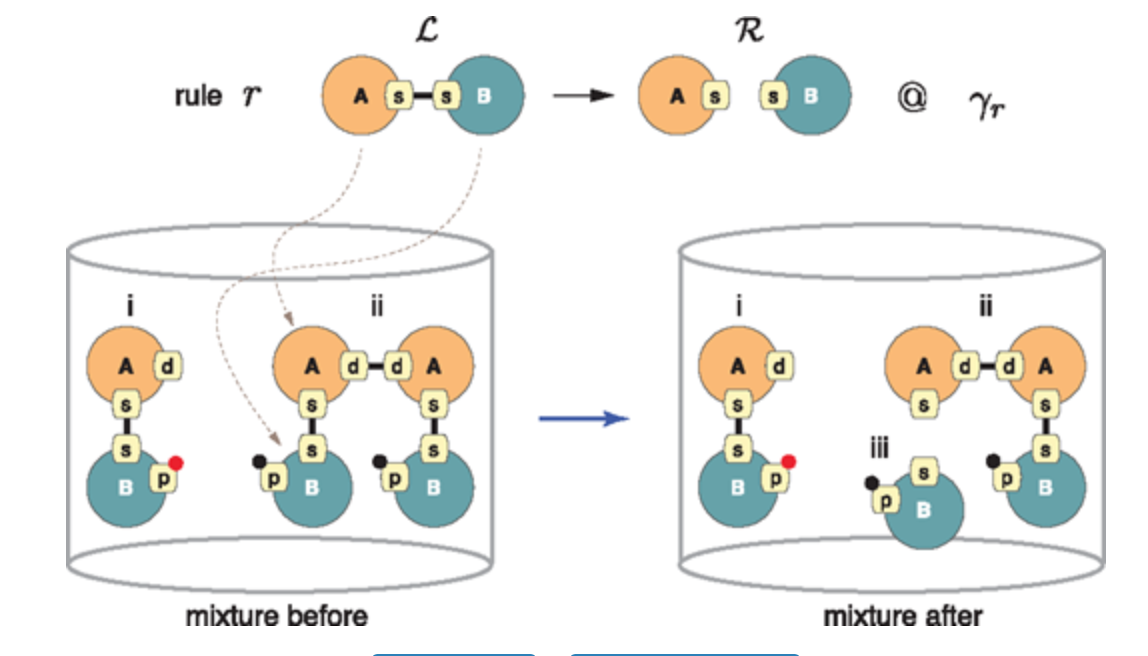
\includegraphics[width=\linewidth,height=10cm,keepaspectratio]{mixture.png}	
	\caption{Application of rule `r' to a reaction mixture \textswab{M}. $L$ and $R$ represent the state of the site graph before and after the application of rule `r'  respectively. Source: \cite{kappaPlatform}}
	\label{fig:mixture}
\end{figure}

Modeling tools built using latest technology help to visualize the protein interactions and simulate the dynamics of the protein complex. Some examples of this include Virtual Cell \cite{vcell} and Kappa Simulator KaSim \cite{kasim}, which provide an environment for the modeling and simulation of cellular interactions. The Kappa rules can be fed into KaSim, which is a protein interaction simulator that implements continuous time Monte–Carlo algorithm (CTMC). Similarly, the rules created in BioNetGet \cite{bioNetGen} format can be simulated with NFsim \cite{nfsim}. KaSim and NFsim employ the process of stochastic modeling that can be used to describe highly complex interactions. Besides them, there also exist other stochastic modeling tools like STOCHSIM \cite{stochsim}, and some others.

In addition to KaSim, the Kappa simulator, there are tools like KaSA (Kappa Static Analyzer) and KaSTOR (Kappa Story Extractor). As per \cite{kappaPlatform}, KaSA helps in analyzing the static properties of the model that can help in debugging, as it can efficiently detect discrepancies between actual and expected behavior. KaSA relies on a technique called `abstract interpretation' described in \cite{kappaPlatform} to achieve this task. KaSTOR helps by providing an insight as to how an event of interest EOI was obtained in a particular event trace. EOI is obtained by the simulation of a model. KaSTOR works on the concept of mechanistic causality in molecular systems. KaSim generates an output called `trace' which is a sequence of events generated as a result of the simulation. Algorithms such as the one stated in \cite{danos2012graphs} aid this process. This is dealt in greater detail, in the Analysis of KaSim outputs, subsection.

\subsection{Syntax and semantics of Kappa rules}
Kappa rules are formally documented well. Their specification and syntax can be found in \cite{kasim} and \cite{kappaURL}. In rule-based specifications, graphs are formally specified as objects which have been converted to a notation of textual form, for convenience. As per these rules an agent site denoted  by `s', has a binding state `n' can be specified as s[n]. Here `n' can be any positive integer or may be replaced by a `.', which indicates the site is not bound. In case `n' is a positive integer then it implies that the site is bound to another unique site having the same binding site `n', within the same PPI expression. Hence, a subexpression like, (Agent1 [site1 [1]], Agent2 [site2 [1]] ) indicates that Agent1 is bound to Agent2 through site1 of Agent1 and site2 of Agent2. The protein sites may also have their own internal states which are specified within curly brackets `\{\}'. Hence Agent1(site1\{p\}[.]), implies that Agent1 has an unbound site name site1 that is in an internal phosphorylated state (denoted by `p'). 

Figure \ref{fig:kappa}, depicts the process of obtaining a Protein interaction rule from the textual information of research literature. These rules when passed to KaSim, the Kappa simulator help to visualize the PPI interactions. 

\begin{figure}[H]
	\centering
	\captionsetup{justification=centering}
	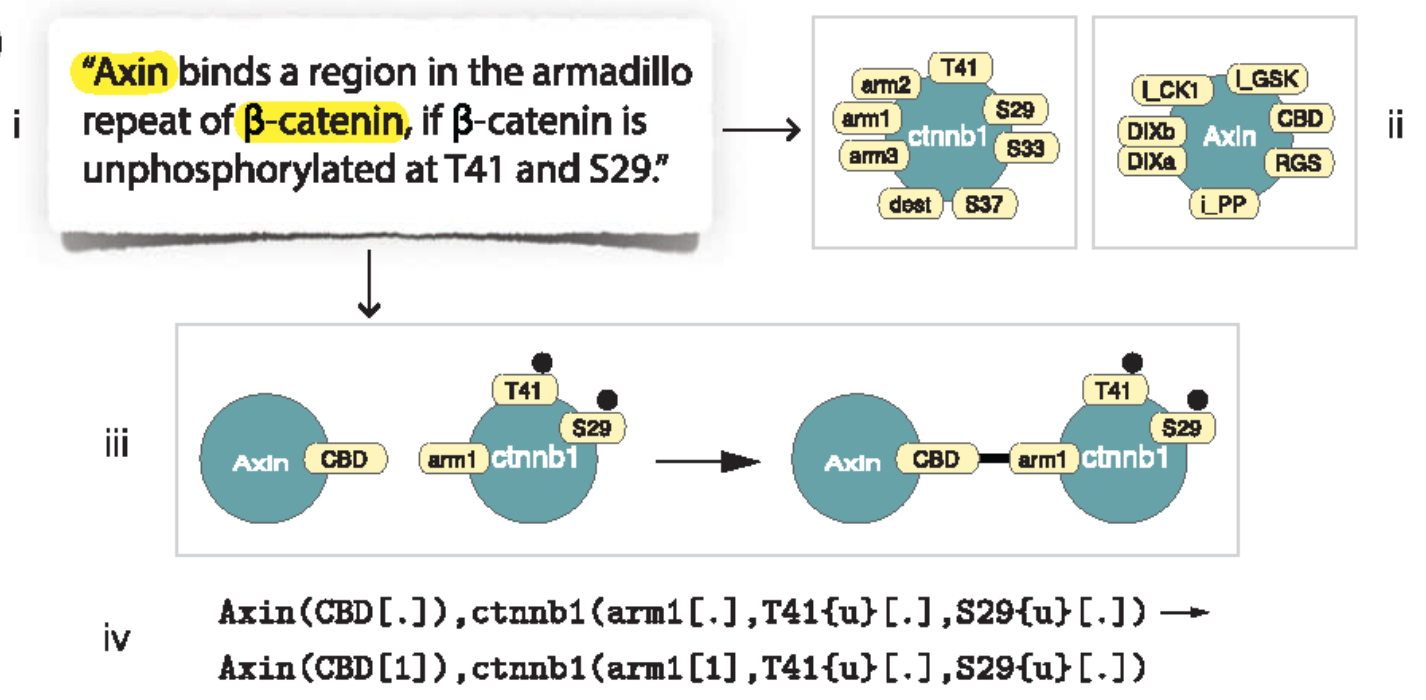
\includegraphics[width=\linewidth,height=10cm,keepaspectratio]{kappa.png}	
	\caption{Depiction of obtaining a Protein-Protein Interaction (PPI) rule from the research literature. Source: \cite{kappaPlatform}}
	\label{fig:kappa}
\end{figure}

\subsection{Analysis of KaSim outputs}
As per \cite{kappaPlatform}, KaSim generates as it's output the whole sequence of events called trace. The analysis of KaSim output includes the discovery of the path by which a particular event of interest (EOI) has occurred. The problem can be formally stated as follows: \\
Provided a trace of events denoted by $\tau$, where $\tau$ = $e_1,e_2,..e_n$ and $e_n$ denotes an individual event. The problem is to find a suitable explanation for an EOI, where the EOI is an event, $e_n \in$ $\tau$ = $e_1,e_2,..e_n$. This process is called causal analysis and in Kappa platform KaSTOR, the software agent is utilized for this purpose. The working of this software and the process of causal analysis is elucidated using the following figure, \ref{fig:eoi}
\begin{figure}[H]
	\centering
	\captionsetup{justification=centering}
	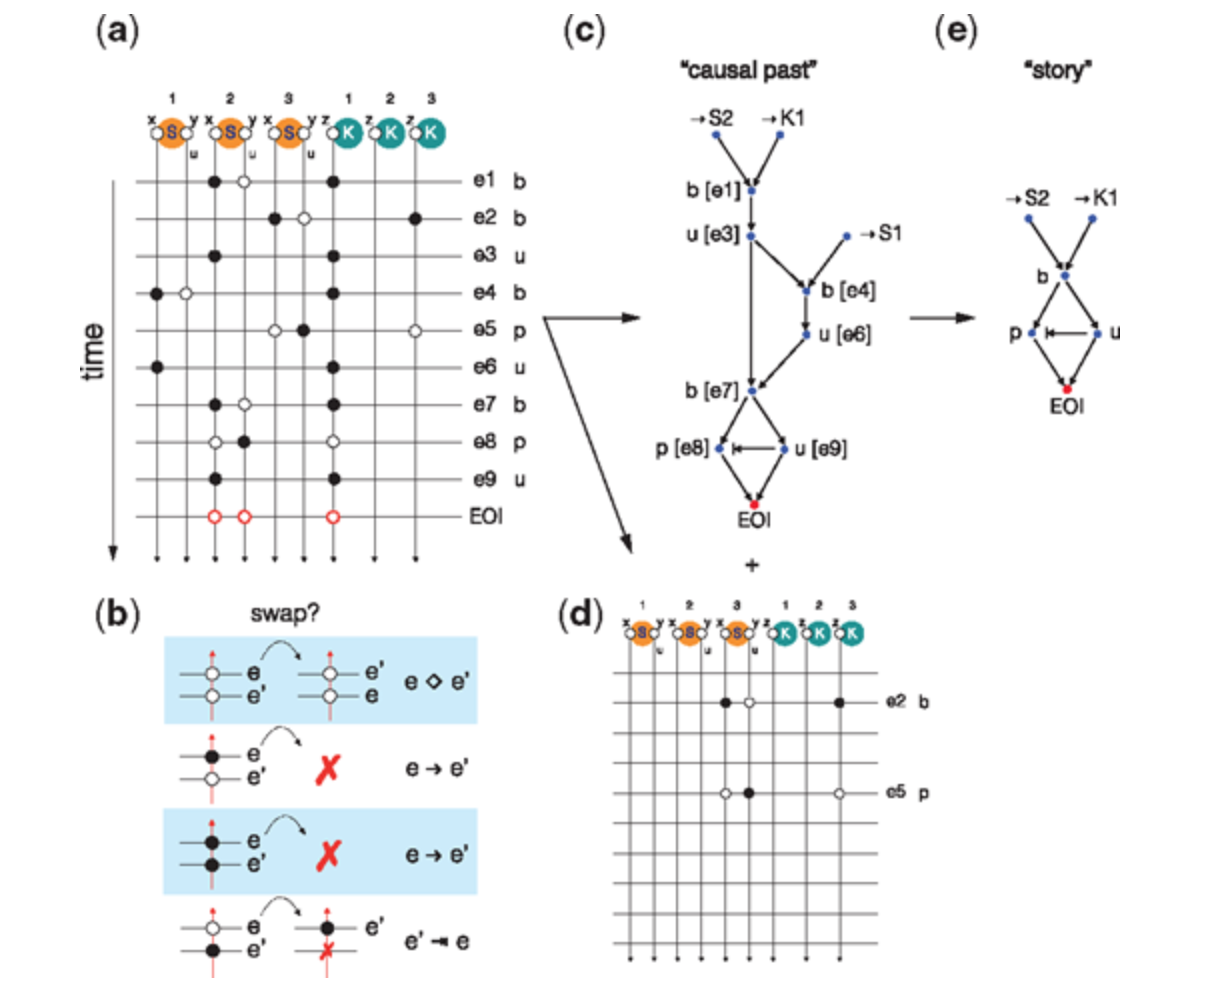
\includegraphics[width=\linewidth,height=10cm,keepaspectratio]{eoi.png}	
	\caption{Explanation of causal analysis. Source: \cite{kappaPlatform}}
	\label{fig:eoi}
\end{figure}

In figure \ref{fig:eoi} (a), the vertical lines from each site, of every agent within the mixture denotes a thread. This thread contains the record whether an event tested or modified the state of a site. It should be noted that in kappa terminology a modification of site also implies a test. The events are shown with the horizontal markings. The black discs denote that the thread was modified by its corresponding horizontal event and the white circle denotes that the thread was tested.

As per \cite{kappaPlatform}, causality comprises of a relation between events. The algorithm begins by reconstructing the causal past of `*', the identity rule. Figure \ref{fig:eoi} (b) depicts an event `e' that is followed by the event ` e$'$ '. and iteratively queries if the modification or test of the site in e$'$  could have occurred before `e'. There are certain rules for the query which are detailed in \cite{kappaPlatform}, under causal linages and compression. This procedure results in a directed acyclic graph (DAG) as shown in \ref{fig:eoi} (c) which represents the precedence structure of the causal past. The procedure depicted in \ref{fig:eoi} (b) also eliminates from within the trace, any events irrelevant to the EOI. This is shown in figure \ref{fig:eoi} (d). The problem with obtaining the precedence structure is that it may violate a property called `necessity'. A method to tackle this problem involves an algorithm called minimization causal compression elaborated in \cite{danos2012graphs}. KasTOR translates the causal past into a boolean expression where each event is associated with a Boolean variable. The processing within KasTOR results to a compressed form of the causal past as shown in figure \ref{fig:eoi} (e).

\section{Applications of Protein-Protein Rule Interaction Database}
The database for PPIs stored in a rule-based format will have several applications. Some of these are covered in this section.
\begin{itemize}
	\item
	\textbf{Building the rule-based model in a Kappa format:} The database will allow collecting in one place the components of already published rule-based models and the new rules based on PPIs. Having that, the database will allow the building of the executable rule-based model, depending on proteins of interest. For that, the list of proteins submitted to the database would result in a list of the relevant rule PPIs retrieved as a CSV file. Those rules could be built into Kappa model and simulated by KaSIM to obtain the dynamics of the respective molecular complex. This would allow the following more specific applications.
	\item
	\textbf{Assessment of protein druggability:} As per \cite{druggability}, ruled based PPI stored in a database is useful in the development of a rule-based model for the assessment of protein druggability. Selection of target is an important step for the discovery of drugs. The effectiveness of a drug target depends upon factors like  its chemical influence and biological importance. Druggability is defined as the ability of a target to bind a drug-like molecule with an affinity that is at a therapeutically useful level. \cite{druggability} develops a set of simple rules that govern the process of druggability which can be applied in the future to get an idea of the chemical influence of prospective targets. These rules are based on the property space of druggable pockets like volume, depth and so on.
	\item 
	\textbf{Drug effect pathway analysis:} Pathway analysis involves the study of specific molecular pathways using formalism that is qualitative and quantitative. This domain provides tremendous computational complexity and experimental approaches that incur a high cost. Research conducted in \cite{ruleMultiscale}, included extraction of about 200 rules, related to type 2 diabetes obtained from varied sources like literature, pathway databases and conversion from different kinds of models. Using these rules \cite{ruleMultiscale} a multi-scale rule-based modeling platform was constructed. This modeling platform was then used for simulation of drug effect pathways of type 2 diabetes drugs and check for its efficacy. The research concluded that their simulation helped in identifying effective drug combinations and provide a new way to effectively apply existing drugs for new targets.
	\item
	\textbf{Application of rule-based models in biology:} Rule-based models can be applied to describe the dynamics of the population in a predator-prey ecosystem and simulate rhythm changes that are circadian \cite{rule_based}.
\end{itemize}

All these research applications help in substantiating the claim that database for storing PPI in a rule format is an important tool for the study the protein complexes, drug discovery and pathway analysis aimed to improve our understanding of complex biological systems.
 

\chapter{Methodology}
This chapter includes the methodology adopted for the creation of rule-based Protein-Protein Interaction (PPI) database and the steps to add a new rule to it. It also contains a description of the stored procedures used to extract protein interaction rules based on either the agent name or a pair of domain names. The source code for this project is available on an online repository (Github). This chapter contains a description of the files and folder structure within it. 

As a part of this project, a web application using Django \cite{django} was created to access the PPI rules by calling the stored procedures from within it. Chapter 3 includes the design and implementation details for the web application used to access the PPI rules. The PPI rules can be accessed from the web application, either based on the agent name or a domain name pair. 

This chapter also includes the steps for deploying the database scripts to a database server and the web application to a web server. During the process of deployment, it is often useful to have the software versions that were initially used to create the software. These are included in Appendix A, under the Software Version section. Having these details will enable developers to debug when deploying the application.

\section{Methodology for creating the database}
PPI rules were collected and provided by researchers in the form of an Excel Sheet (rule\_baseV0.2.xlsx). To extract the agent, domain names and rules from the dataset, excel sheet parser scripts were created in Python. Python scripts were also written to create and validate entity relations within the database. Descriptions of these scripts are elucidated in Section: Description of the Project Folder and Files.

To construct the PPI database it was decided to structure the data into separate tables consisting of the agent, domain and the PPI rules. To connect the data in these three main tables, 2 relationship tables consisting of domain\_agent and rule\_domain\_agent were created.

 It should be noted that the main tables contain certain `metadata columns'. These metadata columns help in keeping track of the associated data for an entity within the table. For example, the domain table has an agent\_name column, which keeps a record of all the agent\_names that it associates to. However, the correct procedure to obtain the agent\_names that associate with a particular domain is to use the domain\_agent relationship table. The Entity Relationship (ER) diagram of the database and the description of the database tables are presented in the following sections.
  \subsection{Entity Relationship Diagram}
  \begin{figure}[H]
  	\centering
  	\captionsetup{justification=centering}
  	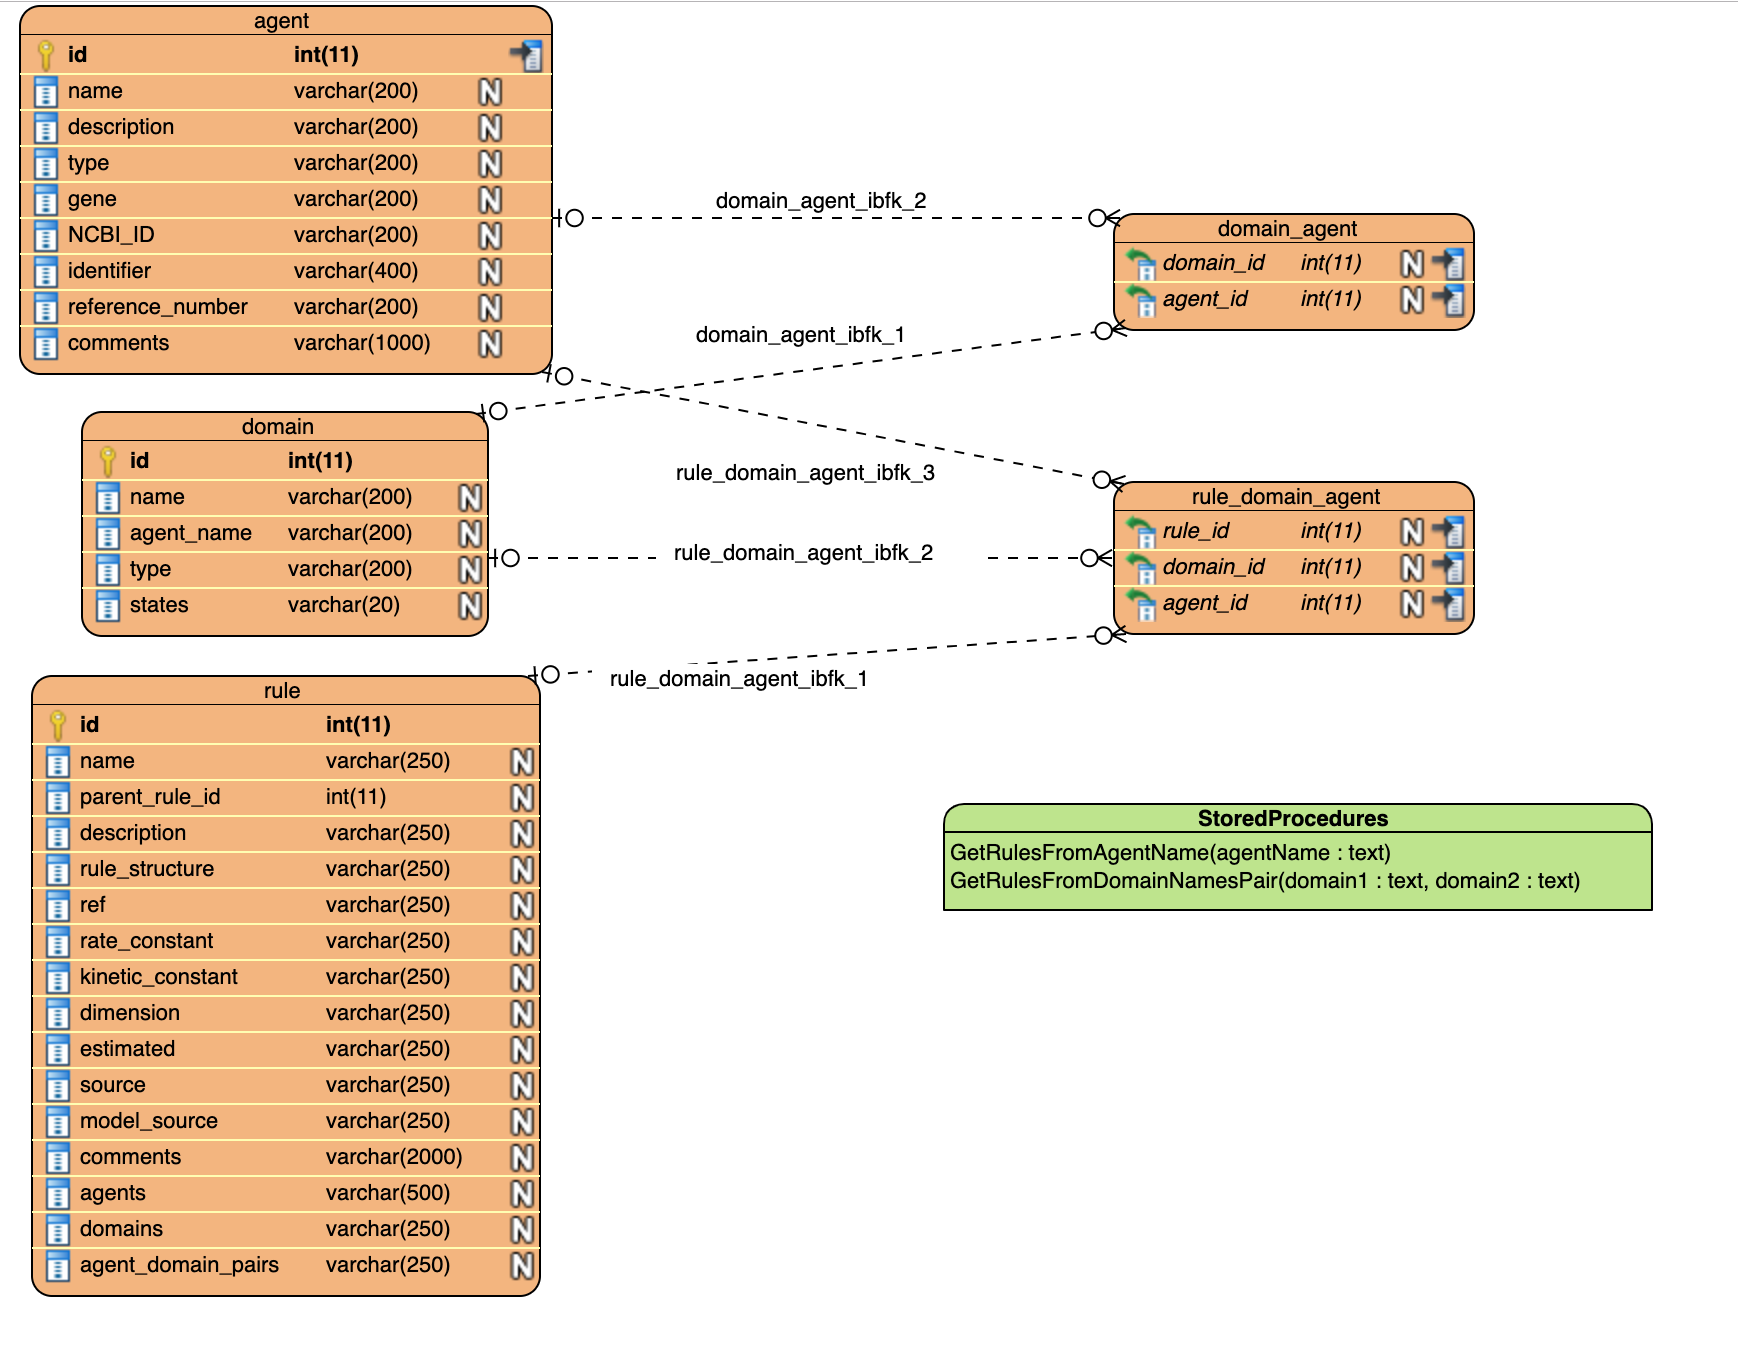
\includegraphics[width=\linewidth,height=14cm,keepaspectratio]{er.png}	
  	\caption{Database ER Diagram created using software Visual Paradigm \cite{vd}}
  	\label{fig:er}		
  \end{figure}
  In Fig \ref{fig:er}, the dotted lines depict the primary-foreign key relations between the tables. The green box depicts the names of the stored procedures that are part of the database.
 \subsection{Description of  main tables}
\begin{enumerate}
	\item \textbf{agent:-} Describes the protein molecule (the agent). This table contains the following fields: id, name, description, type, gene, NCBI\_ID, identifier, reference\_number and comments.
	\begin{enumerate}
		\item id: The unique identifier for the agent molecule.
		\item name: The name of the agent.
		\item description: A description of the agent.
		\item type: The type/family of the agent.
		\item gene: The particular gene
		\item NCBI\_ID, identifier, reference\_number: Provided within the dataset and contains references to the Uniprot Prosite Database \cite{Uniprot-Prosite} and literature.
		\item comments: Contains additional comments about the agent.
	\end{enumerate}
	\item \textbf{domain:-}  Describes the domains that associate with the agents. This table contains the following fields: id, name, agent\_name, type, states. 	
		\begin{enumerate}
		\item id: The unique identifier for the domain name.
		\item name: The name of the domain.
		\item agent\_name: A `metadata column' that contains the names of agent molecules that associate with the particular domain.
		\item type: The type of the domain.
		\item states: Contains the possible states of the domain.
	\end{enumerate}
	\item \textbf{rule:-} Provides a description of the PPI rules within the database. 
	This table contains the following fields: id, name, parent\_rule\_id, description, rule\_structure, ref, rate\_constant, kinetic\_constant, units, estimated, source, model\_source, comments, agents, domains and agent\_domain\_pairs.
	\begin{enumerate}
	\item id: The Unique identifier for the rule
	\item name: The name of the rule
	\item parent\_rule\_id: In some cases the rules can be traced to a parent. This field stored the id of that parent rule. By default it is 0, which signifies no parent rule.
	\item description: A description of the rule.
	\item rule\_structure: The structure of the rule. 
	\item ref, source: A reference to the rule.
	\item rate\_constant: The rate constant for the reaction.
	\item kinetic\_constant: The kinetic constant may contain numerical value or a formula to which the rate\_constant can be plugged to obtain the result.
	\item dimension: The units for the kinetic constant
	\item estimated: The estimated value of the constant.
	\item model\_source: A reference to the model from which the PPI is obtained.
	\item comments: Any additional comments about the rule.
	\item agents: A `metadata column' containing the names of the agent molecules that take part in the rule.
	\item domains: A `metadata column' containing the names of the domains that take part in the rule.
	\item agent\_domain\_pairs:	A `metadata column' containing the names agent and associated domains that form a part of the protein interaction.
	\end{enumerate}
\end{enumerate}

 \subsection{Description of  relationship tables}
\begin{enumerate}
	\item \textbf{domain\_agent:-} Each row contains the id of a domain and the id of an agent, obtained by referencing the domain and agent table respectively. 
	By obtaining the domain id from the domain table, the corresponding agent ids that associate with the domain can be obtained. This can then be used to obtain the agent names that associate with that particular domain.
	\begin{enumerate}
		\item domain\_id: The Id of a domain (from domain table).
		\item agent\_id: The Id of an agent (from agent table).
	\end{enumerate}

	\item \textbf{rule\_domain\_agent:-} Each row contains the id of a rule, id of a domain and the id of an agent, obtained by referencing the rule, domain and agent table respectively. Hence, this table connects the agents and domains to the PPI rules from the rule table in the database.
	\begin{enumerate}
		\item rule\_id: The Id of a rule (from rule table).
		\item domain\_id: The Id of a domain (from domain table).
		\item agent\_id: The Id of an agent (from agent table).
	\end{enumerate}
\end{enumerate}
 \subsection{Advantages and  disadvantages of the database structure}
 \subsubsection{Advantages}
The database structure is optimized for fast read operations. This is because, by using the id structure to uniquely identify entities in the database, we can leverage the power of indexing \cite{indexing}, which can be used to obtain the results faster. As per \cite{indexing}, in section 8.3.1, most MySQL indexes like primary key, unique key are stored in B Trees. Due to this, it is possible to obtain rows matching the where clause quickly and even leverage the power of Multiple-Column Indexes, as per \cite{indexing} section 8.3.6. It was also verified in MySQL workbench that the relationship tables (domain\_agent and rule\_domain\_agent) had each of the columns indexed as a B Tree. Hence MySQL would internally be able to work more efficiently with this structure than we if we employed a method that included string regex-based searching.
 \subsubsection{Disadvantages}
 The disadvantage of this database design is that it makes the write operations a multi-step process. For example, if we wanted to add a new rule to the database then besides performing the regular checks, several entries may have to be made in different tables within the database. This is however not a major disadvantage as the database is expected to have many more read operations than write, also the next section states the steps to add a new PPI rule to the database. While trying to make a new entry within the database, following these rules will help in reducing the errors.
\section{Steps for adding new entries to the database}
\subsection{Agent}
	Query the agent table and check if an agent exists with the given name. It should be noted that the agent name is case sensitive. In case it exists then there is no need to add a new entry to the database. However, if it does not exist then a new entry can be made in the agent table filling in the relevant fields. 
\subsection{Domain}
	Query the domain table and check if a domain exists with the given name. It should be noted that the domain name is case sensitive. In case it exists then there is no need to add a new entry to the database. However, if it does not exist then a new entry can be made in domain table filling in the relevant fields. 
\subsection{Domain-Agent}
	When the Agent/Domain is added to the database to connect them we have to make entries within the domain\_agent table. Based on the entries made in the Agent and Domain table we can obtain the corresponding ids and make entries containing the (domain id, agent id) pairs. If a new agent is added then all its corresponding domains need to be entered as separate rows where the agent id will remain the same. If a new domain is added then all its corresponding agents need to be added as separate rows where the domain id will remain the same. 	
	It should be kept in mind that if a new agent is added to the agent table and it has a new corresponding domain added to the domain table, then that pair must be entered only once within the domain\_agent table.	
\subsection{Rule}
	To add a new rule to the database, first, check if the rule already exists within the database. If not, then obtain the agents and domains that take part in the rule. Verify that the necessary agents, domains and domain\_agent entries exist within the database. If not, then first make the necessary entries in these three tables as per guidelines in the previous sections. Then add the PPI rule to the rule table in the database. 
	\subsection{Rule-Domain-Agent}
	After following the steps laid out in Rule subsection, the three pair tuple/s consisting of the rule\_id, agent\_id for each of the agents in the rule and the domain\_id for each of the domains that associate with the corresponding agent within rule, need to be entered in the rule\_domain\_agent table as (rule id, domain id, agent id).
\section{Description of Stored Procedures}
 In Fig \ref{fig:er}, the green box displays stored procedures defined within the database. The two stored procedures created are GetRulesFromAgentName and GetRulesFromDomainNamePair. The expected input, output and algorithm for each of the stored procedure is mentioned in the following subsections.
 \subsection{GetRulesFromAgentName}
 \textbf{Input:} An agent name (data type: text).\\
 \textbf{Output:} PPI rules in which the agent name, provided as an input occurs.\\ 
 \textbf{Algorithm} 
 \begin{enumerate}
 	\item The agent id corresponding to the agent name is obtained from the agent table. 
 	\item A list of the rules, in the form of rule ids occurring along with the agent id (obtained in step 1) is extracted from the rule\_domain\_agent table. This is a list of distinct rule ids, which implies that none of the rule ids are repeated in the output.
 	\item Using the list of distinct rule ids, the rules are extracted from the rule table and provided as the output of the stored procedure.
 \end{enumerate}
 \subsection{GetRulesFromDomainNamesPair}
  \textbf{Input:} Two domain names (data type of each being: text).\\
 \textbf{Output:} PPI rules in which both the domain names, provided as an input occurs.\\ 
 \textbf{Algorithm}
  \begin{enumerate}
 \item  The domain id for each of the domains is extracted from the domain table and stored in two separate variables within the stored procedure, called domain1 and domain2. 
\item  From the table, rule\_domain\_agent those rule ids are extracted that co-occur with the domain2.
\item  The rule ids are extracted which co-occur with domain1 and also occur in the list of rule ids extracted in the previous step. Hence implying that the rules ids occurring in this step are the rules that co-occur with domain1 and domain2. This is a distinct list of rule ids. 
\item Using the list of distinct rule ids, the rules are extracted from the rule table and provided as the output of the stored procedure.
 \end{enumerate}
\section{Description of the project folder and its files}
\subsection{Project folder source}
This project is hosted on Github, as a public repository in the link \cite{sourceCode}, and is open source.
\subsection{Project folder structure and files}
The main folder is called PPI\_DB, which contains within it the following sub-folders:
 \begin{enumerate}
 	\item Django-app: Contains files of the web application for accessing the PPI rules. The relevant files and folder structure are elucidated in the next section.
 	\item Parser: Contains files pertaining to extracting the agents, domains and PPI rules from the dataset (rule\_baseV0.2.xlsx). This folder has the following files and sub-folder.
 	\begin{enumerate}
 		\item PARSER\_POPULATE\_TABLE\_AGENT.py: Accesses the Agents Sheet of the dataset and generates the table insertion script for the  SQL table, agent.
 		\item PARSER\_POPULATE\_TABLE\_DOMAIN.py: Accesses the Agents Sheet of the dataset and generates the table insertion script for the SQL table, domain.
 		\item PARSER\_POPULATE\_TABLE\_RULE.py: Accesses the Rules Sheet of the dataset and generates the table insertion script for the SQL table, rule.
 		\item Extractors: This folder contains python scripts used to obtain the agents, domains, agent-domain pairs and kinetic constants for each of the PPI rules, from the Rules Sheet of the dataset. These extracted columns are then appended to the Rules Sheet of the dataset, as additional columns and included into the SQL rule table. The `metadata columns' like agents, domain and agent-domain pairs provide additional information about the rules.
 		\item DB\_POPULATE\_TABLE\_DOMAIN\_AGENT.py: This script connects to the database using the credentials mentioned within the script and generates the table insertion script for the SQL table, domain\_agent. 
 		
 		To summarize, this script works by first obtaining a row from the domain table created in step (b). The agent\_name field in the row gives names of all the agents to which the domain associates itself with. The id of each of these agents is obtained from the agents table and the id of the domain is included in the row extracted from the domain table. Then insert table commands of the form (domain\_id, agent\_id) are generated, to populate the domain\_agent table.
 		\item DB\_POPULATE\_TABLE\_RULE\_DOMAIN\_AGENT.py: This script connects to the database using the credentials mentioned within the script and generates the table insertion script for the SQL table, rule\_domain\_agent. 
 		
 		To summarize, this script works by first obtaining a row from the rule table created in step (c). The agent\_domain\_pairs field in the row gives all the agent-domain pairs within that PPI rule. The id of each of these agents is obtained from the agents table and the id of the domain is obtained from the domain table (both obtained by querying from the database). Then insert table commands of the form (rule\_id, domain\_id, agent\_id) are generated, to populate the rule\_domain\_agent table.
 	\end{enumerate}
 	\item Stored Procedure: Contains two files that define stored procedures.
 	\begin{enumerate}
 		\item RULES\_FROM\_AGENT\_NAME.sql: Defines the stored procedure that returns the PPI rules based on the agent name as input.
 		\item RULES\_FROM\_DOMAIN\_NAME\_PAIR.sql: Defines the stored procedure that returns the PPI rules based on the pair of domain names as input.
 	\end{enumerate}
 
 	\item Table Populate Scripts: Contains database scripts that are used to populate the PPI database. These table insertion scripts are written in MySQL format and tested using the MySQL client called MySQLWorkbench. It contains the following files:
 	 	\begin{enumerate}
 		\item AGENT.sql: Script to populate the agent table.
		\item DOMAIN.sql: An initial Script to populate the domain table. (included in the projects file only for reference).
		\item DOMAIN\_V2.sql: Script to populate the domain table.
		\item RULE.sql: Script to populate the rule table.
		\item DOMAIN\_AGENT.sql: Script to populate the domain\_agent table.
		\item RULE\_DOMAIN\_AGENT.sql:  Script to populate the rule\_domain\_agent table.
 	\end{enumerate}
 
 	\item Tables/Database Creation Scripts: Contains the database scripts used to define and create the database and tables within it. These scripts are written in MySQL format and tested using the MySQL client called MySQLWorkbench. It contains the following files:
 	 	 	\begin{enumerate}
 		\item CREATE\_DATABASE\_PPI.sql: Script to define and create the PPI Database. This serves as a container to store the PPI database tables.
 		\item CREATE\_TABLE\_AGENT.sql: Script to define and create the agent table.
 		\item CREATE\_TABLE\_DOMAIN.sql: Script to define and create the domain table.
 		\item CREATE\_TABLE\_RULE.sql: Script to define and create the rule table.
 		\item CREATE\_TABLE\_DOMAIN\_AGENT.sql: Script to define and create the domain\_agent table.
 		\item CREATE\_TABLE\_RULE\_DOMAIN\_AGENT.sql:  Script to define and create the rule\_domain\_agent table.
 	\end{enumerate}
 
 \item Rectified Rules:  Verification steps were adopted after the initial population of the database. A report was generated based on any discrepancies within the data in the database. For example, it is possible that while inserting a rule it is observed that the domain that the agent occurs with was not entered in the database before as it was not observed in the Agents sheet, in the dataset. Based on the report and subsequent discussions the table population scripts were updated. More information regarding the verification pipeline is presented in the `Results and Discussion Section'. This folder contains the following two files:
    \begin{enumerate}
   	\item problematic\_agents\_domains.txt: The initial report on the observed discrepancies.
   	\item rule\_baseV0.2\_fixed.xlsx: The dataset with the updated values for agents, domains and rules based on the discrepancies reported in\\ problematic\_agents\_domains.txt. It is an updated version of the dataset contained in the Parser folder.
   \end{enumerate}
 \end{enumerate}
	
\section{Web Application for accessing the stored procedures}
This section provides a walk-through of the Django app file structure and the important files for the project. It also explains the procedure to run the Django app and retrieve the PPI rules. We also explain the functionality of the user interface (UI) in this section.
\subsection {Folder Structure and files}
Files for the web application are contained in the Django-app folder within the source code hosted on Github repository, \cite{sourceCode}. The root folder for Django app is called djangonautic and within it, we find the  subfolders called djanjonautic, ppi and templates. This folder also contains the manage.py file which is automatically generated while creating the Django app and is used to run tasks like making database migrations and starting the webserver. 

Within the djangonautic folder contains an important file called settings.py. This contains important information such as the installed apps and database connection details. In case the django-app needs to be extended then the installed app need to be registered in the INSTALLED\_APPS section. The database details can also be modified from the settings.py file in the DATABASES section.

The ppi folder contains the files and templates relevant to extracting and displaying the PPI information in the webpage. When the URL is invoked, to serve the client request the Django server first matches the URL with the URL patterns available in the urls.py file located in this folder. Once the URL pattern is matched, the corresponding function from the views.py file is invoked. Within the functions of the views.py file, the database call to the relevant stored procedure is made. Once the result is returned by the database the relevant template from the ppi/templates folder is invoked and the result is rendered onto the screen. The static folder within the ppi/templates contains the javascript, css and fonts obtained from the library \cite{dataTables}, are used to create and display the PPI rules in the UI. 
\subsection {Running the web application}
In order to run the web application the following steps need to be performed:
 \begin{enumerate}
 	\item  The SQL server in which the database is hosted should be in running state. In MAC OSX this can be verified by navigating to the System Preferences $\to$ MySQL and ensuring that the MySQL server is running. 
 	\item Navigate to the folder django\_app $\to$ djangonautic and run the following command to start the server.\\
 	python manage.py runserver
 \end{enumerate}
\subsection {Get PPI rules based on agent name}
\begin{enumerate}
	\item In order to access the PPI rules based on Agent Name, enter the following URL in the web browser: http://127.0.0.1:8000/ppi/AgentNameForm/.
	\item Enter the agent name in the text box provided and click on submit as shown in the figure \ref{fig:agentNameForm}. (Note: The agent name is case sensitive). Internally the Django application makes a connection to the database and invokes the GetRulesFromAgentName stored procedure and passes the agent name as an argument to it.
	\item The retrieved PPI rules will be visible in the next page as shown in figure \ref{fig:agentNameRules}. In case there are no matching PPI rules then a message is displayed on the screen to inform the user.
\end{enumerate}
  \begin{figure}[H]
	\centering
	\captionsetup{justification=centering}
	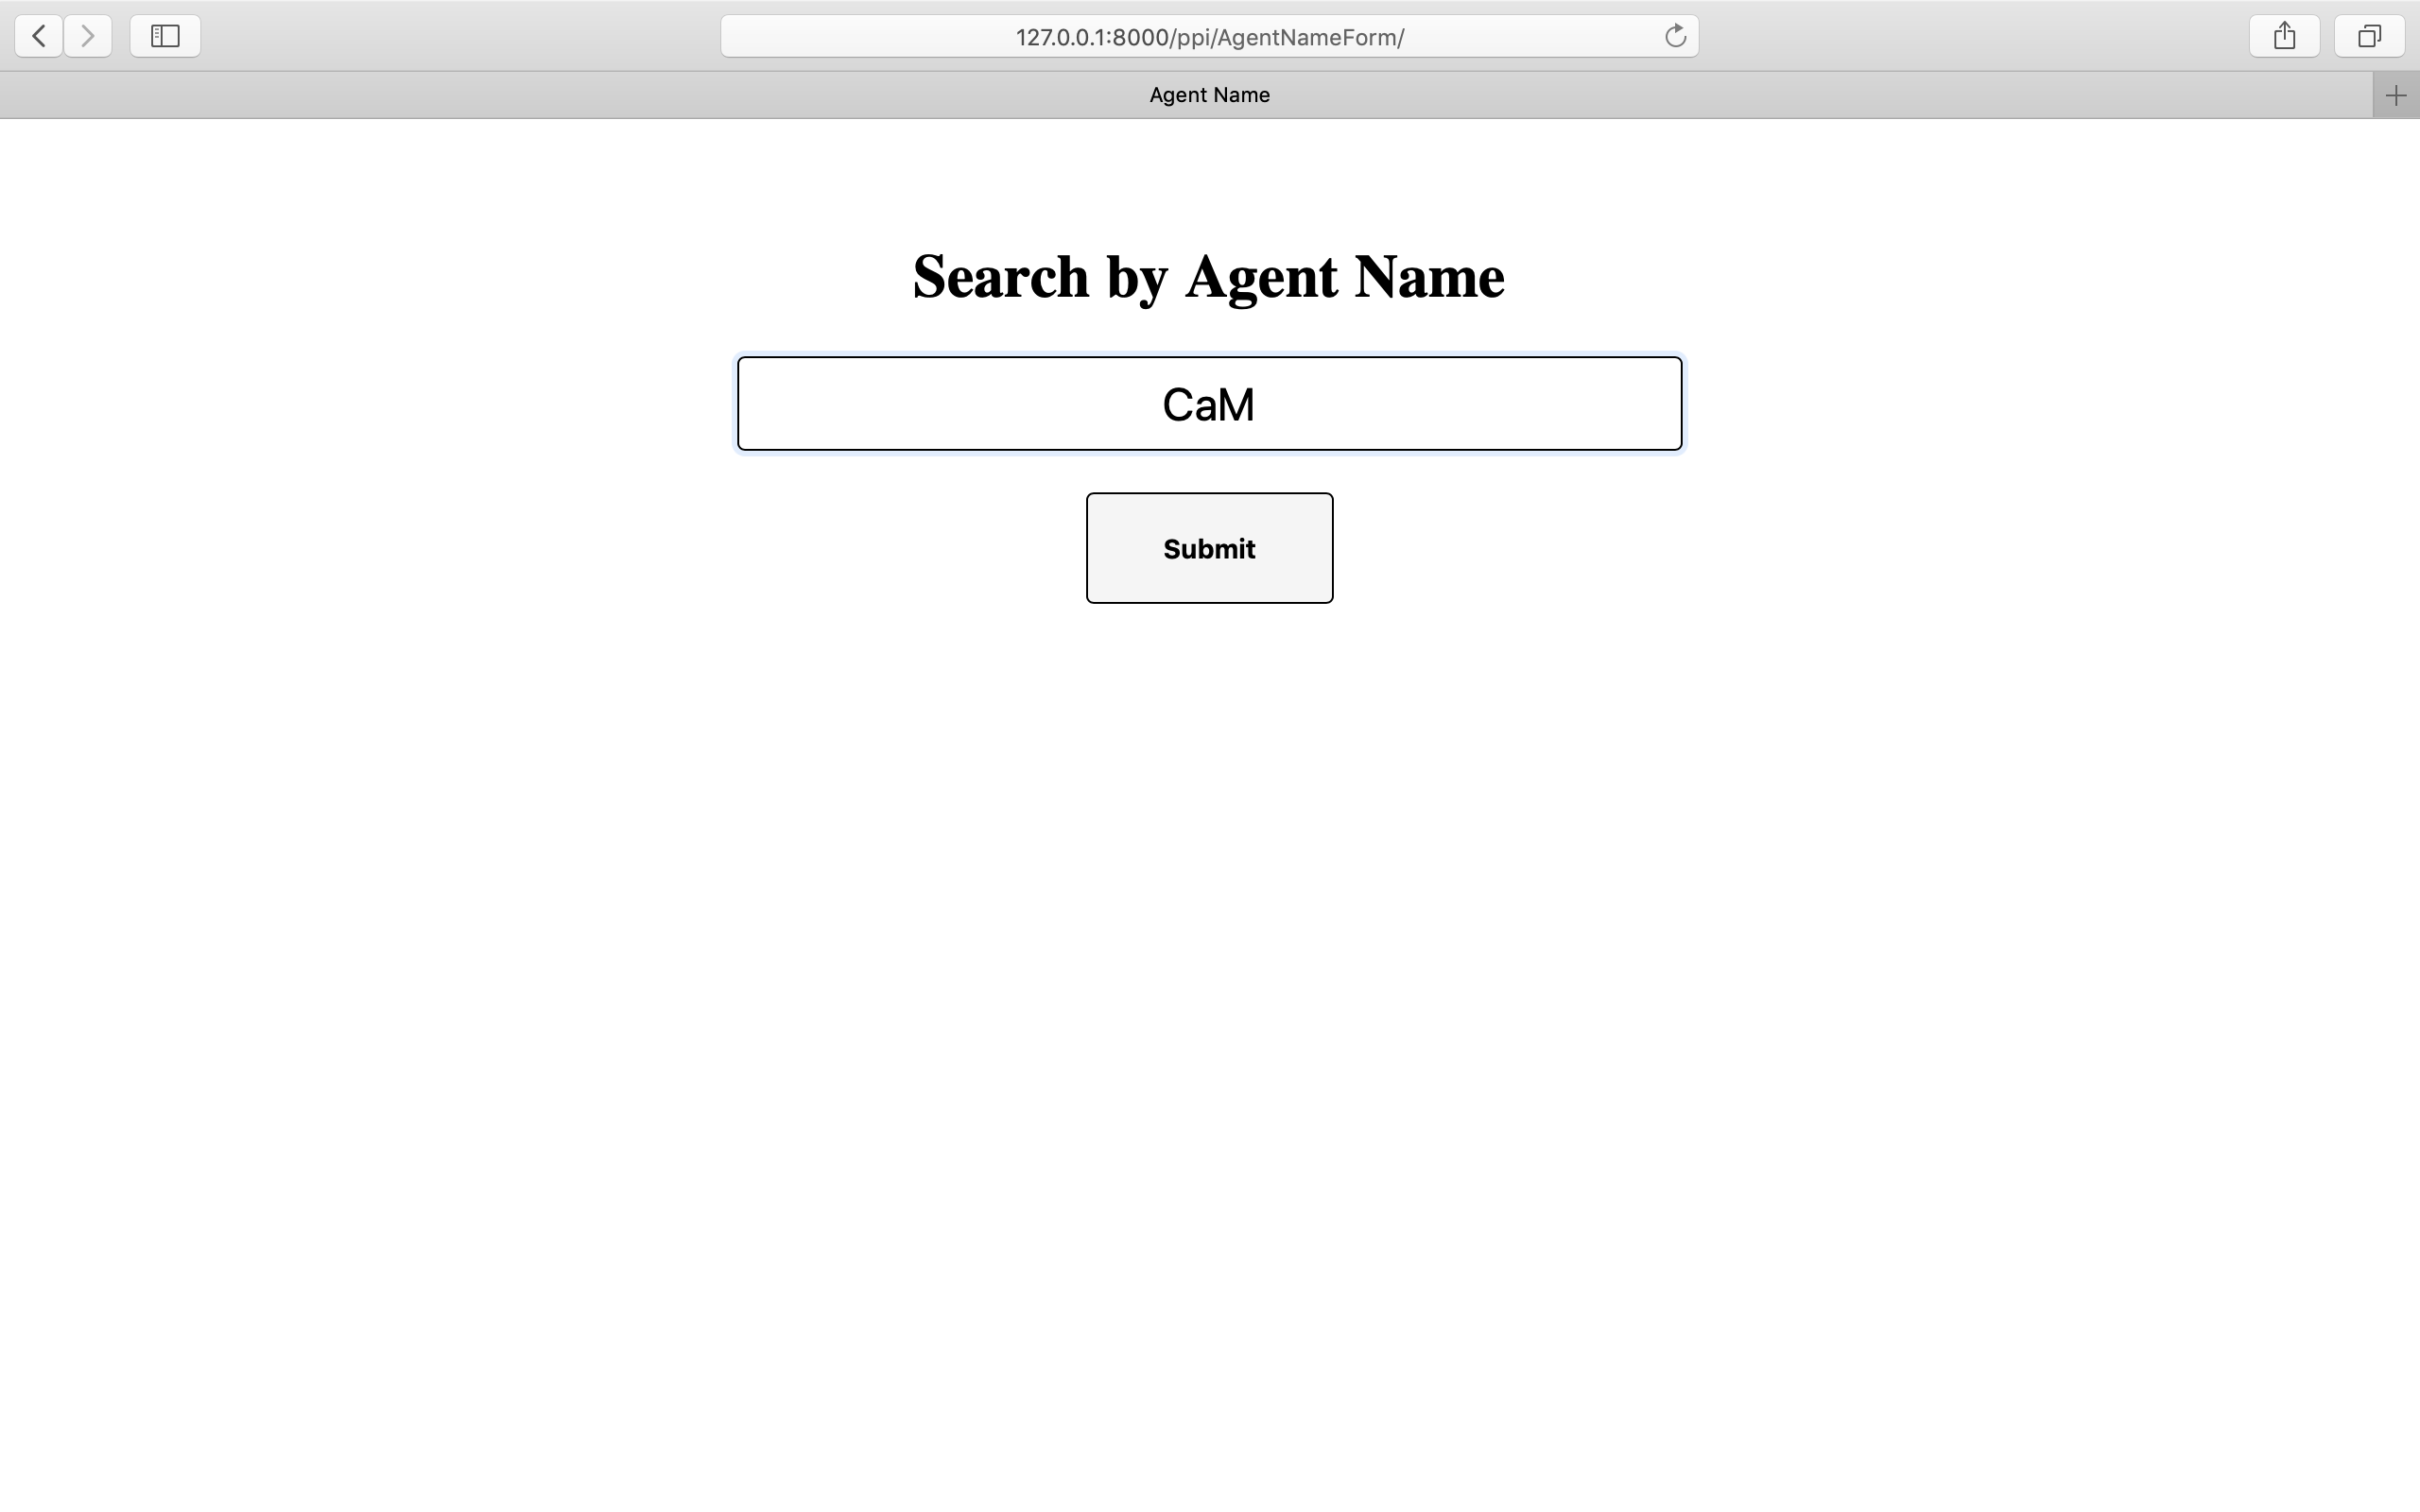
\includegraphics[width=\linewidth,height=14cm,keepaspectratio]{AgentNameForm.png}	
	\caption{Form to accept the agent name.}
	\label{fig:agentNameForm}		
\end{figure}

  \begin{figure}[H]
	\centering
	\captionsetup{justification=centering}
	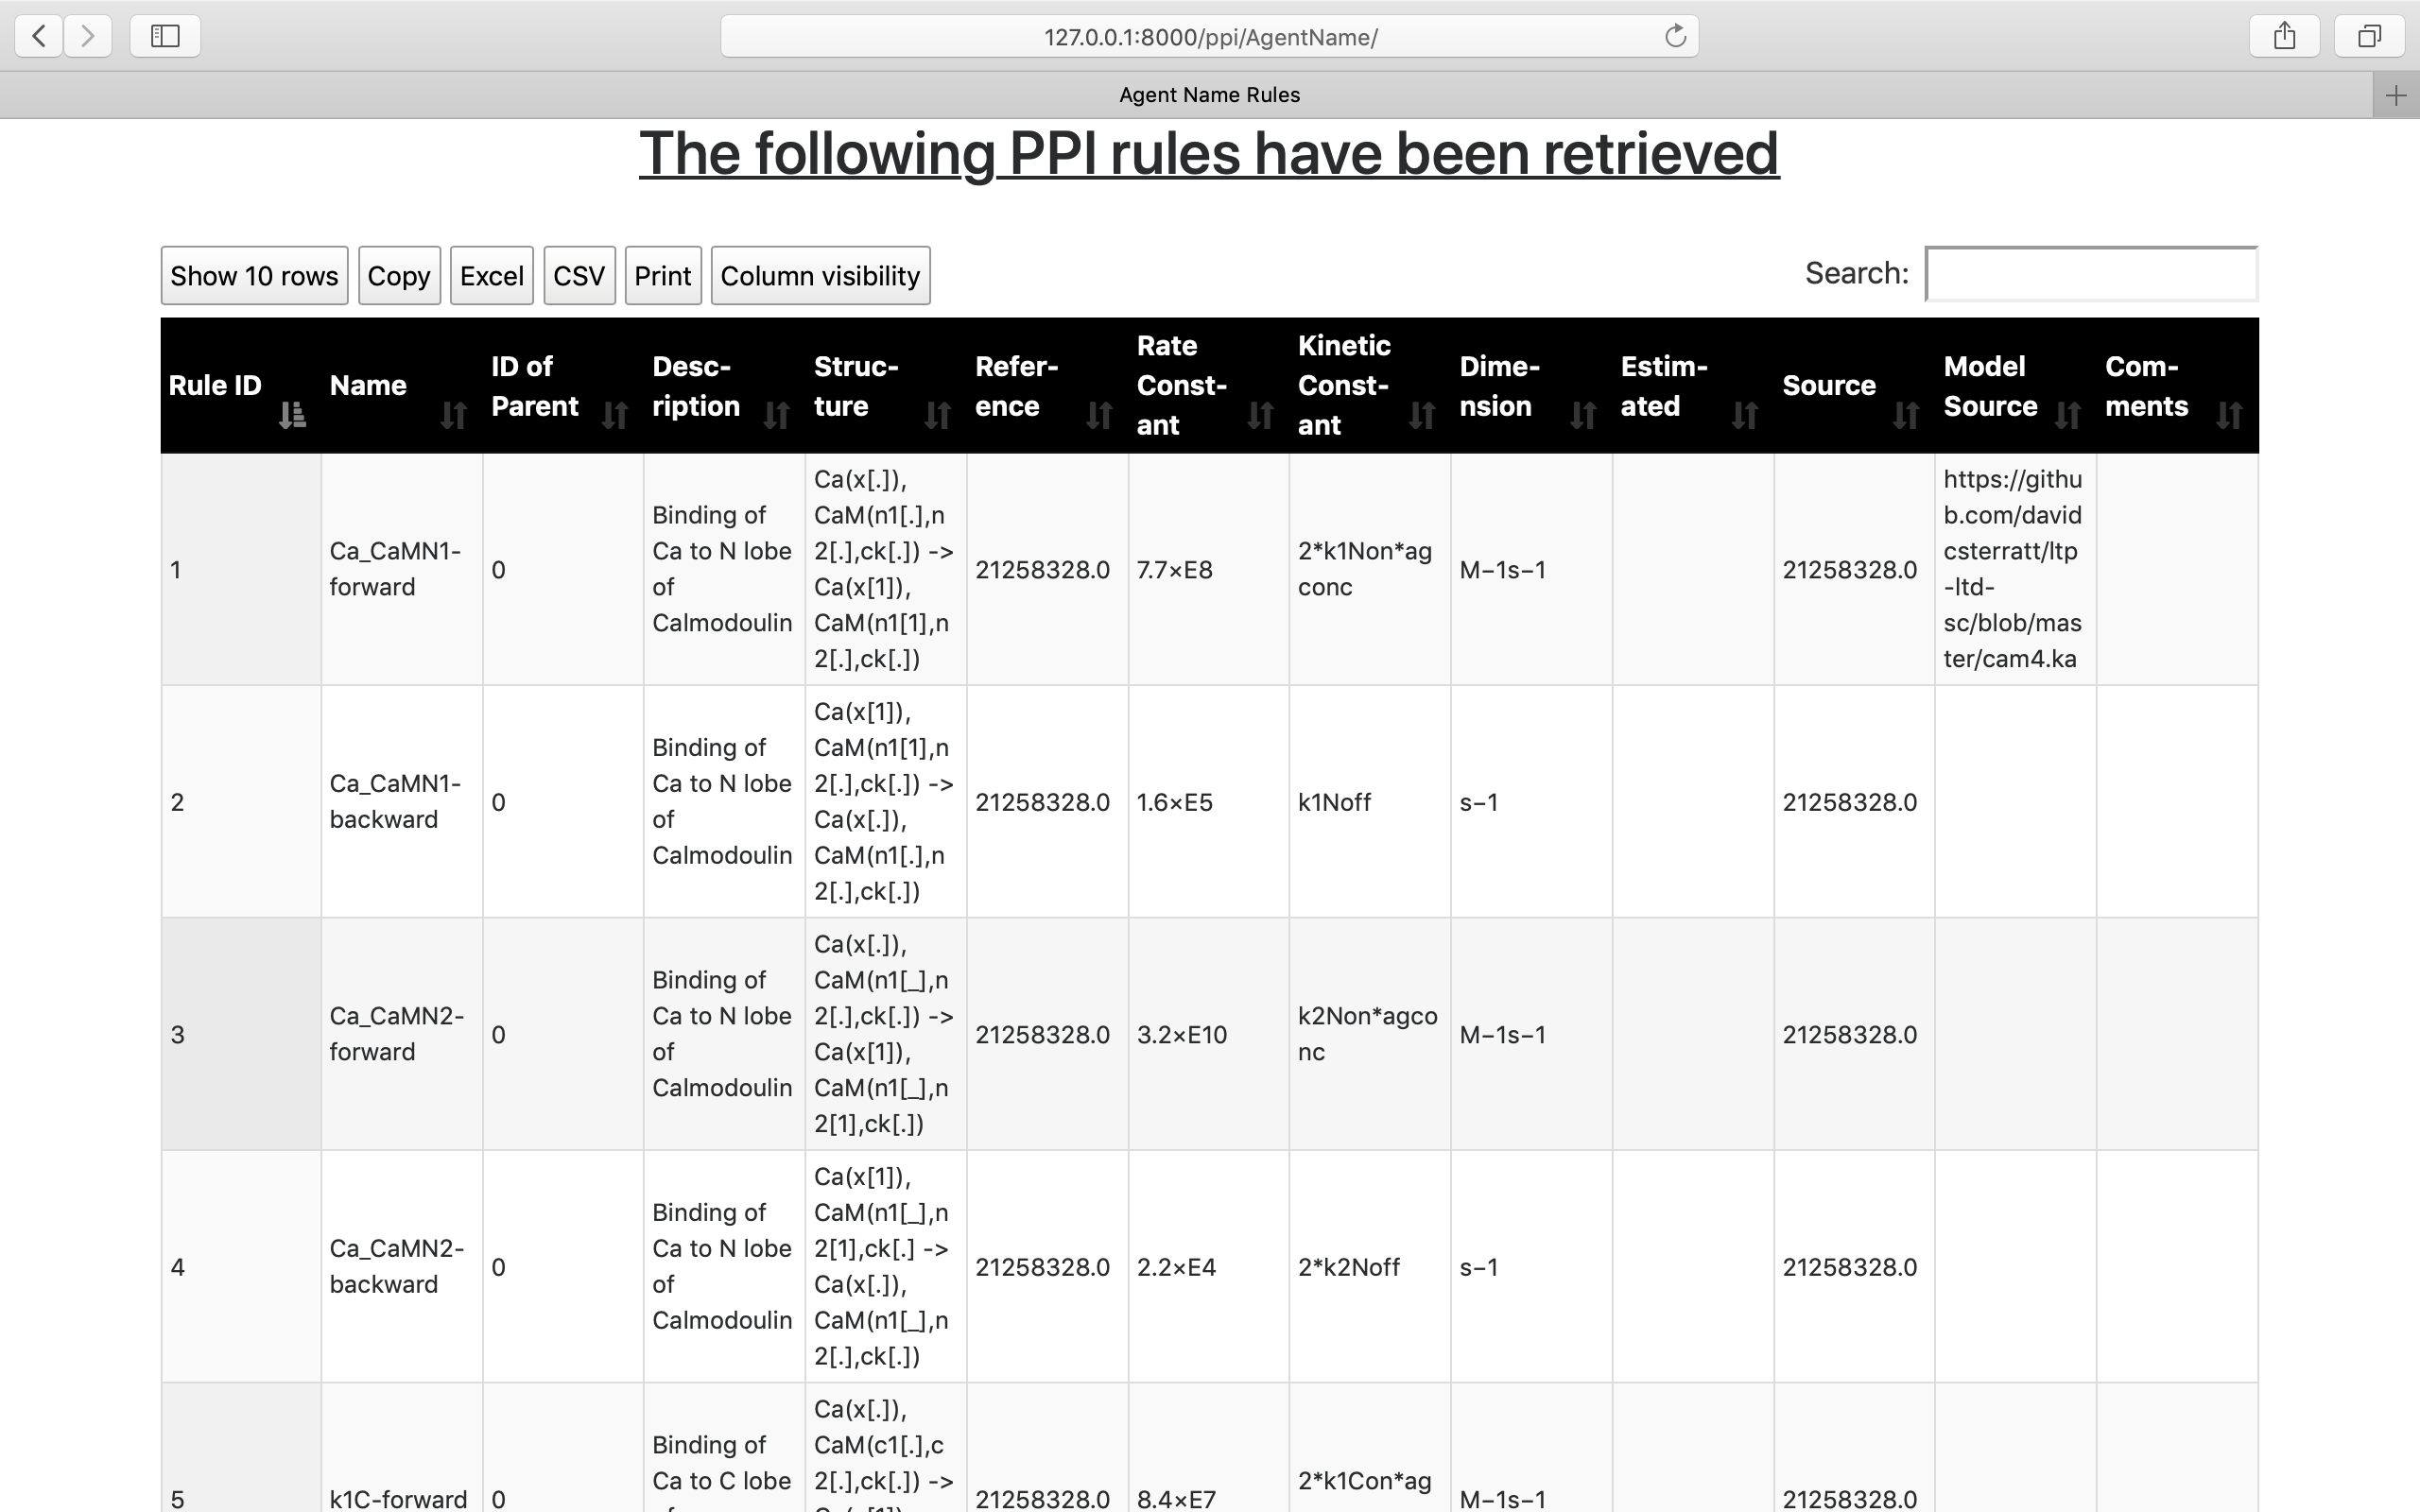
\includegraphics[width=\linewidth,height=14cm,keepaspectratio]{AgentNameRules.png}	
	\caption{The rules retrieved based on the agent name provided in the agent name form.}
	\label{fig:agentNameRules}		
\end{figure}

\subsection {Get PPI rules based on domain names}
\begin{enumerate}
	\item To access the PPI rules based on a pair of domain names, enter the following URL in the web browser: http://127.0.0.1:8000/ppi/DomainNameForm/
	\item Enter the domain names in the text boxes provided and click on submit, as shown in figure \ref{fig:domainNameForm}. (Note: The domain names are case sensitive). Internally the Django application makes a connection to the database and invokes the GetRulesFromDomainNamePair stored procedure and passes the domain names as arguments to it.
	\item The retrieved PPI rules will be visible in the next page as shown in figure \ref{fig:domainNameRules}. In case there are no matching PPI rules then a message is displayed on the screen to inform the user.
\end{enumerate}
	 \begin{figure}[H]
		\centering
		\captionsetup{justification=centering}
		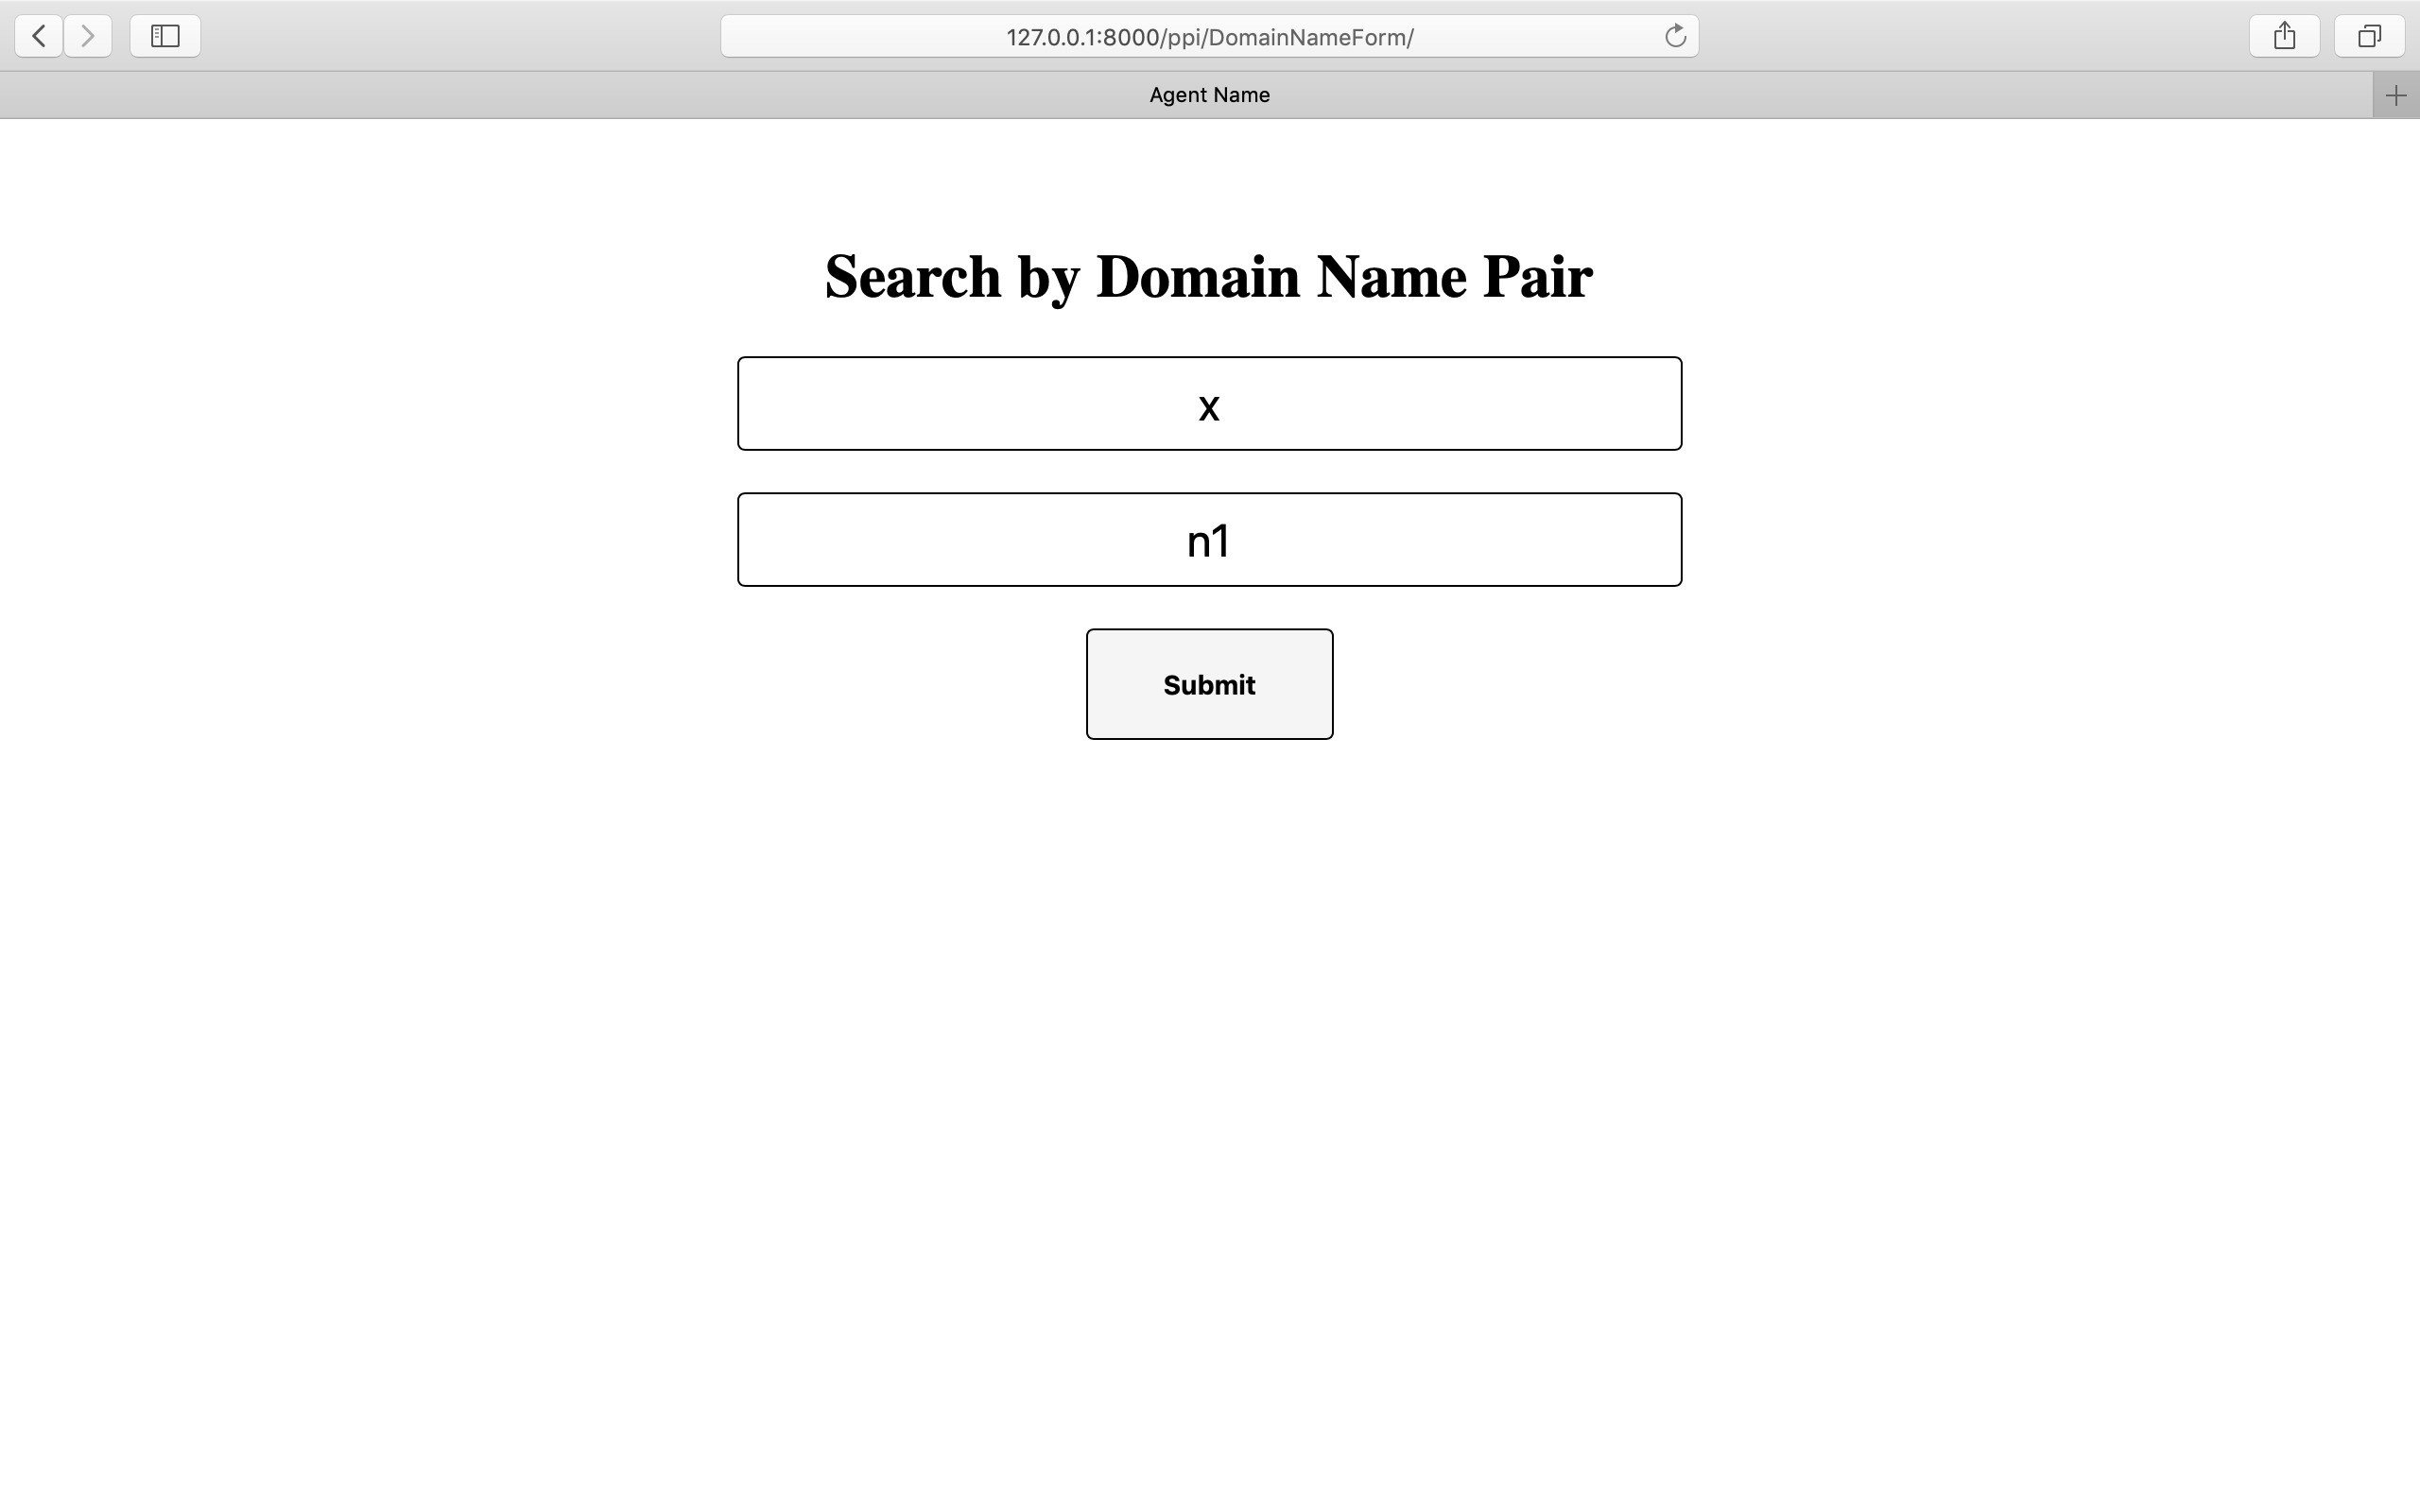
\includegraphics[width=\linewidth,height=14cm,keepaspectratio]{DomainNameForm.png}	
		\caption{Form to accept the domain names.}
		\label{fig:domainNameForm}		
	\end{figure}
\begin{figure}[H]
	\centering
	\captionsetup{justification=centering}
	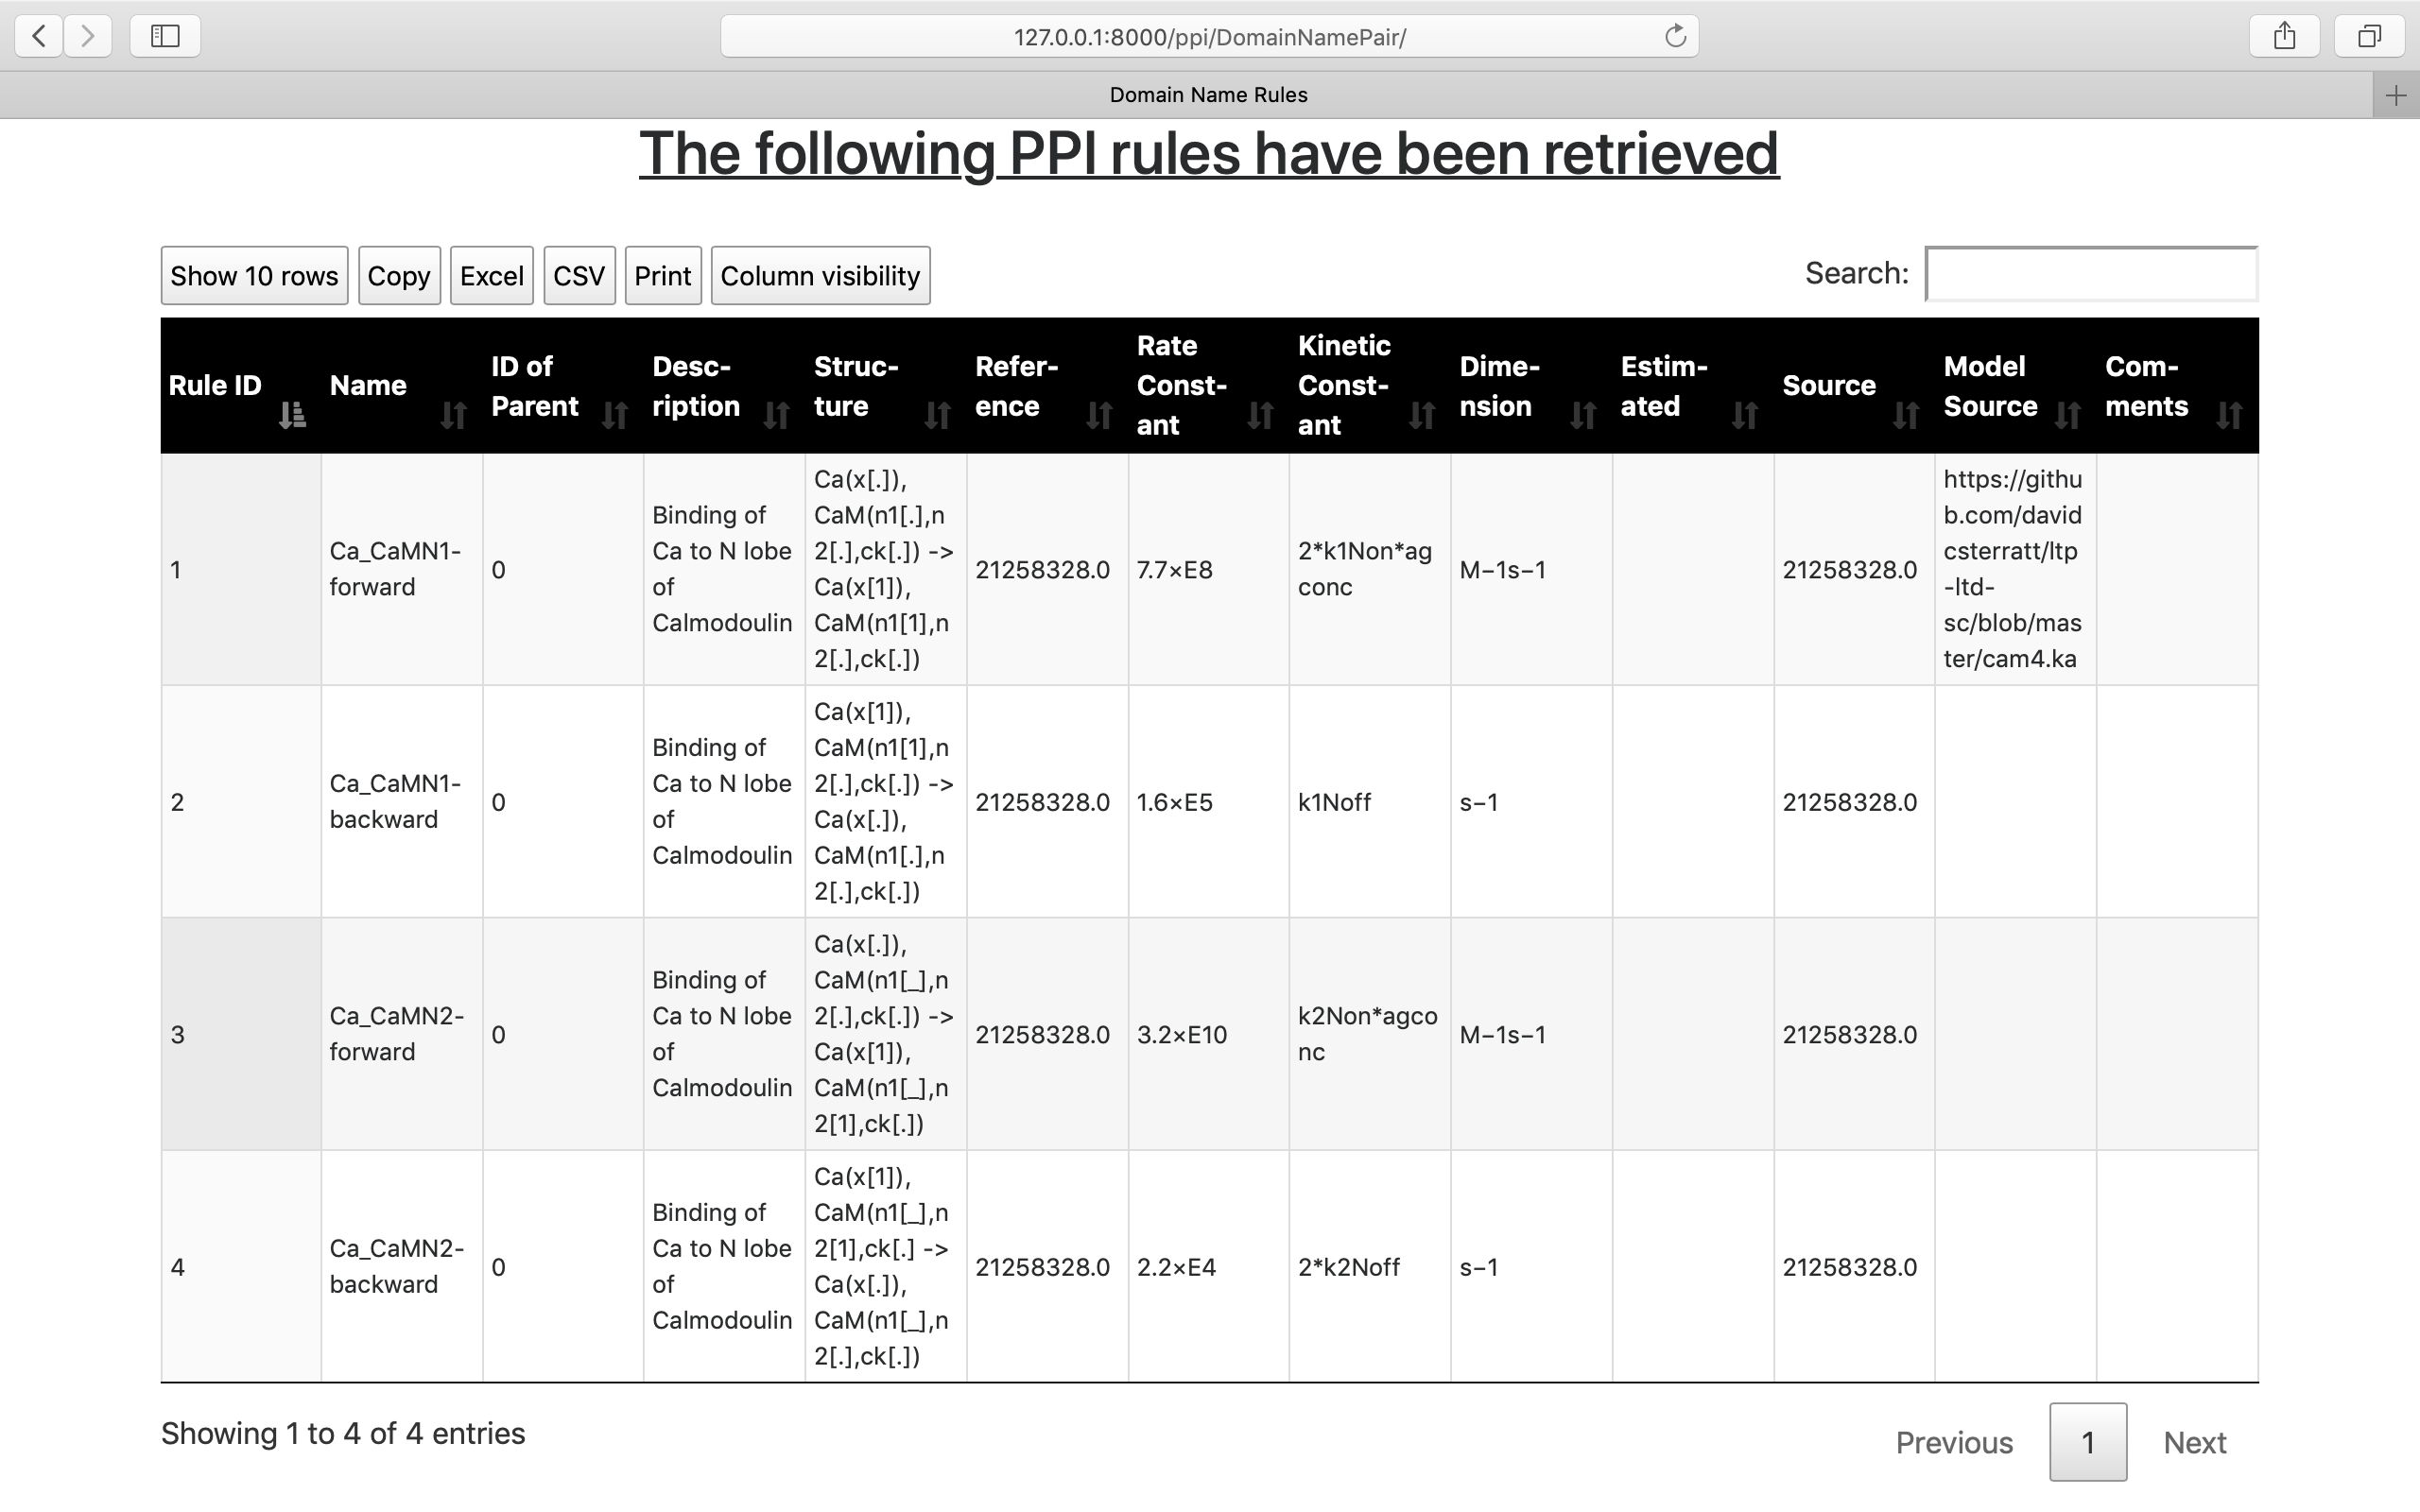
\includegraphics[width=\linewidth,height=14cm,keepaspectratio]{DomainNameRules.png}	
	\caption{The rules retrieved based on the domain names provided in the domain names form.}
	\label{fig:domainNameRules}		
\end{figure}

\subsection {User Interface (UI) functionality}
The buttons in the user interface have been created with the help of the DataTables library \cite{dataTables}. These UI options are helpful, as the retrieved results can be processed and fed into the  kappa simulator for visualization of the protein interactions. A description of the buttons in figure \ref{fig:UI} is as follows:
\begin{figure}[H]
	\centering
	\captionsetup{justification=centering}
	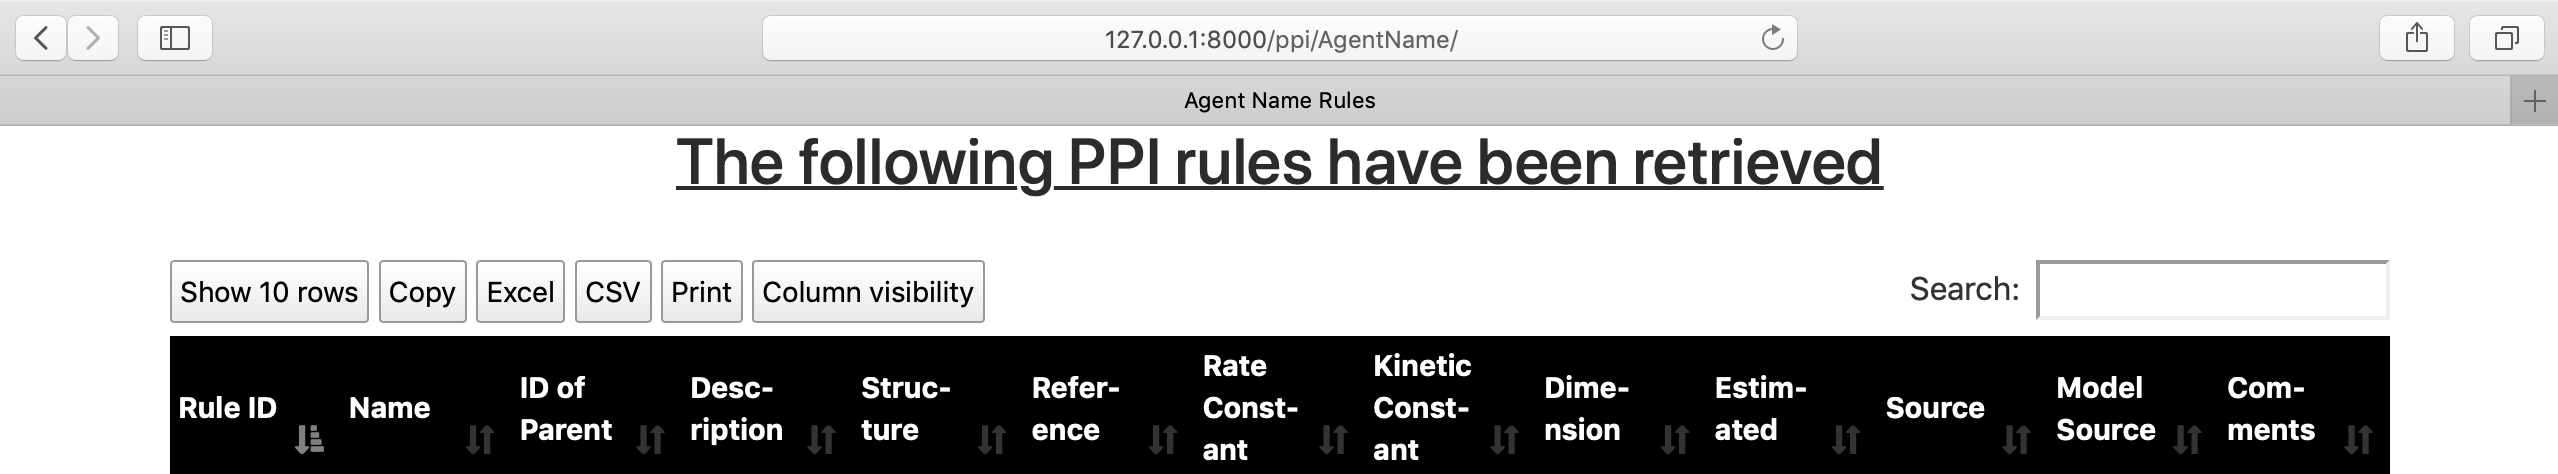
\includegraphics[width=\linewidth,height=14cm,keepaspectratio]{UI.png}	
	\caption{A closer view at the user interface (UI) buttons.}
	\label{fig:UI}		
\end{figure}
\begin{enumerate}
	\item Show `n' rows: Provides the option of displaying 10, 25, 50, 100 or all the rows.
	\item Copy: Allows the table to be copied to the clipboard.
	\item Excel: Allows the table to be exported to an excel sheet.
	\item CSV: Allows the table to be exported to a file where the data entries are separated by a comma.
	\item Print: Allows the user to print the retrieved results.
	\item Column visibility: Allows the user to decide which columns are to be visible. This can be useful while exporting or saving only the required results.
	\item Arrow buttons beside the field names: Allow the user to sort the results in numerical order in case of a numerical field or alphabetical order in case of a text field.
	\item Search: The search button allows the user to search over the entire table based on a search key.
\end{enumerate}
\section{Deployment steps}
\subsection{Database Scripts}
 The SQL scripts were tested on MySQL server using the client MySQLWorkbench. The respective versions can be found in Appendix A. To deploy the database scripts onto a database server the following steps need to be followed.
 \begin{enumerate}
 	\item Create a user account within the database server (if not created already).
 	\item Login to the user account within the database server.
 	\item Navigate to the Tables:Database Creation Scripts folder located within the project folder hosted on Github. 
 	\item Execute the CREATE\_DATABASE\_PPI.sql SQL script in the MySQL client, to create the PPI database.
 	\item Execute the remaining scripts in the following order, CREATE\_TABLE\_AGENT.sql, CREATE\_TABLE\_DOMAIN.sql, CREATE\_TABLE\_DOMAIN\_AGENT.sql, CREATE\_TABLE\_RULE.sql and CREATE\_TABLE\_RULE\_DOMAIN\_AGENT.sql.
 	\item Navigate to the Table Populate Scripts folder located within the project folder hosted on Github.
 	\item Execute the SQL scripts in the following order AGENT.sql, DOMAIN\_V2.sql, RULE.sql, DOMAIN\_AGENT.sql and RULE\_DOMAIN\_AGENT.sql.
 \end{enumerate}
\subsection{Web Application}
To deploy the web application onto a web server navigate to the django\_app folder within the project folder hosted on Github.
\begin{enumerate}
	\item Navigate to the file django\_app/djangonautic/djangonautic/settings.py, update the database credentials with the ones created in the previous section, in the DATABASE section of the code and save it.
	\item Navigate to the folder django\_app/djangonautic/ and run the following commands to synchronize the data models within the django application, with the database:\\
	python manage.py migrate \\
	python manage.py makemigrations
	\item After synchronizing the data model, start the webserver by running the following command:\\
	python manage.py runserver\\
	and access the URLs for retrieving the PPIs based on agent name or domain names through a web browser.	
\end{enumerate}
The web application was tested on the web browsers Safari, Google Chrome and Mozilla Firefox.
\chapter{Verification and Results}
This chapter presents the verification techniques adopted, to ensure correctness in several parts of the project. These include aspects of correctness in database creation, values retrieved by the stored procedures and the displayed results within the UI. It also presents an example output from KaSim (the simulator), when fed with PPI rules.
\section{Verification pipeline for database entries}
This section details the verification pipeline used to ensure the correctness of data stored within the PPI database. This is verified using the following reasoning and python scripts within the project folder.
\begin{enumerate}
	\item The Agent table is created by parsing the Agents sheet within the provided dataset (Excel sheet).
	\item The domain table is then created by parsing the agents sheet within the provided dataset (Excel sheet). Hence the agent table and the domain table is obtained.
	\item The rule table was then created by parsing the Rules sheet within the provided dataset (Excel Sheet). The rules were pre-processed to obtain the agents, domains and agent-domain pairs. These were added as additional columns in the Excel sheet and are visible in the Processed Excel Sheets folder. The additional columns are also visible in the rule table of the database.
	\item The correctness of parsing the rules was manually verified to ensure that they were free from errors. 
	\item We next proceed to create the domain\_agent table using the script\\ DB\_POPULATE\_TABLE\_DOMAIN\_AGENT.py.\\ The script connects to the database and obtains a domain by querying the domain table. It acquires its corresponding id and all the associated agent names from the domain table. 
	\item This script then queries the database for each of the agent names associated with that particular domain. 
	\item In case it does not find the agent name in the agent table of the database, it reports this discrepancy.
	\item In case it finds the agent name in the agent table of the database then it proceeds to create the SQL entry for the domain\_agent table.\\ Note: The domain id was already obtained in step 3. 
	\item We next proceed to create the rule\_domain\_agent table using the script\\ DB\_POPULATE\_TABLE\_RULE\_DOMAIN\_AGENT.py.\\ The script connects to the database using MySQL connector and for each rule, it obtains the agents and domains present within the rule.
	\item  It then connects to the database and queries if each of the agent names exists within the database. In case it does not, then it reports the discrepancy with the prefix Problem in AGENT\_NAME. 
	\item For each of the domains extracted it checks whether the domain name exists in the domain database. In case the domain name does not exist, then it reports this discrepancy with the prefix Problem in DOMAIN\_NAME. These discrepancies are written to a file named problematic\_agents\_domains.txt.
	\item The script then proceeds to verify that an agent and domain extracted from the rule, have the necessary entry in the domain\_agent relation. In case, it does not find this entry, then it reports this discrepancy.
	\item  In case no discrepancies were observed then, it implies that the agent name occurs in the agent database and the domain name exists in the domain database. Also the relevant connection between the domain and agent is found in the domain\_agent relation.
	\item The MySQL table entry for the relation rule\_domain\_agent for the observed rule, domain and agent is created. This procedure is repeated for each of the agents and associated domains within the rule and for every rule.	
	\item Finally, the discrepancies were examined and discussed with the  supervisor. Based on inputs provided the discrepancies were resolved and the database loading scripts were updated to accommodate the changes.
\end{enumerate}
\section{Verification of stored procedure results}
Two stored procedures were created as part of the project. These are useful in retrieving the PPI rules based on the criteria defined in the following sub-sections.
\subsection{GetRulesFromAgentName}
The purpose of this stored procedure is to return the PPI rules which contain the agent name (provided as an input). To verify that the defined stored procedure behaves as expected, test cases were tried and the outputs were verified. Some of these test cases are as follows: 
\begin{enumerate}
	\item 
	\begin{itemize}
		\item 	The stored procedure is called with the agent name `CaM',\\
		using the command, call GetRulesFromAgentName(`CaM') \\
		 from MySQL workbench.
		 \item 	The expected output is the PPI rules, containing the agent CaM within it.
		 \item 	The output obtained from the database contained 14 rows. A snippet of the output is shown below, in figure \ref{fig:AgentNameOutput1}. Each of these PPI rules was verified to contain the agent name CaM within it.\\
	\end{itemize}	
	\begin{figure}[H]
		\centering
		\captionsetup{justification=centering}
		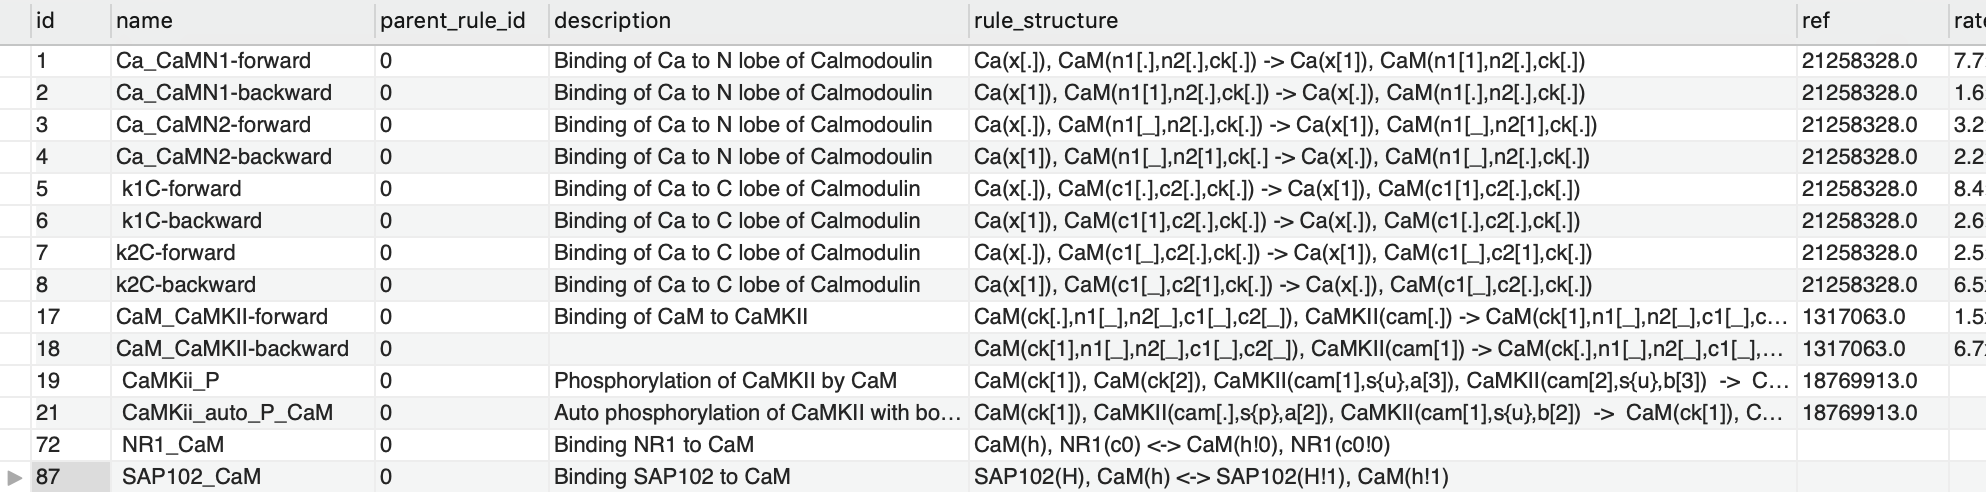
\includegraphics[width=\linewidth,height=14cm,keepaspectratio]{AgentNameOutput1.png}	
		\caption{The retrieved rules from the stored procedure GetRulesFromAgentName called with the argument `Cam'.}
		\label{fig:AgentNameOutput1}		
	\end{figure}

	\item 
	\begin{itemize}
		\item 	The stored procedure is called with agent name `SynGAPa',\\
		using the command, call GetRulesFromAgentName(`SynGAPa')\\
		from MySQL workbench.
		\item The expected output is the PPI rules, containing the agent SynGAPa.
		\item The output obtained from the database contained 6 rows. A snippet of the output is shown in figure \ref{fig:AgentNameOutput2}. Each of these PPI rules was verified to contain the agent name SynGAPa within it.
	\end{itemize}
		\begin{figure}[H]
		\centering
		\captionsetup{justification=centering}
		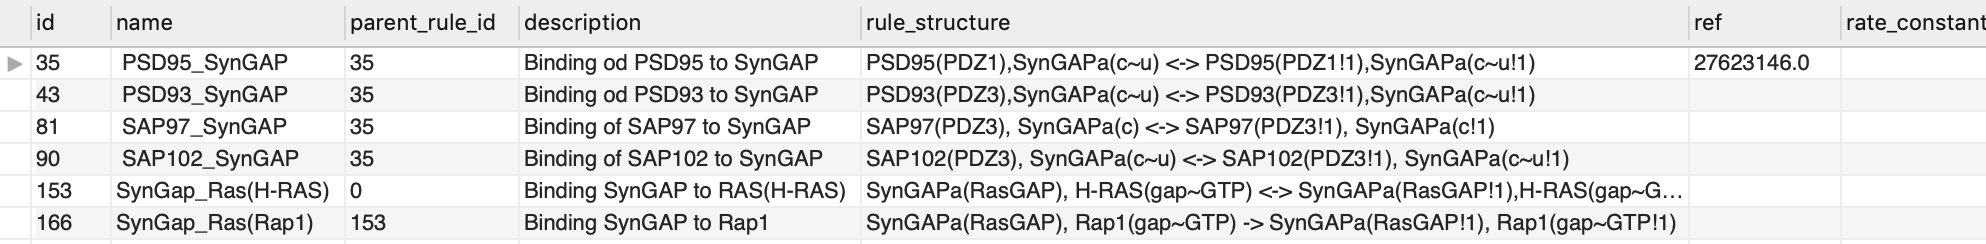
\includegraphics[width=\linewidth,height=14cm,keepaspectratio]{AgentNameOutput2.png}	
		\caption{The retrieved rules from the stored procedure GetRulesFromAgentName called with the argument `SynGAPa'.}
		\label{fig:AgentNameOutput2}		
	\end{figure}
\end{enumerate}

\subsection{GetRulesFromDomainNamesPair}
The purpose of this stored procedure is to return the PPI rules which contain the domain  names (provided as an input). To verify that the defined stored procedure behaves as expected, test cases were tried and the outputs were verified. Some of these test cases are as follows: 
\begin{enumerate}
	\item 
	\begin{itemize}
		\item 	The stored procedure is called with the domain name arguments `x,n1', using the command, \\
		call GetRulesFromDomainNamesPair(`x',`n1')\\
		from MySQL workbench. 
		\item The expected output is the PPI rules, containing the domain names x and n1 within it.
		\item The output obtained from the database contained 4 rows. A snippet of the output is shown below, in figure \ref{fig:DomainNameOutput1}. Each of these PPI rules was verified to contain the domain names x and n1 within it.
		\item The stored procedure call was also tested with the arguments swapped (n1 and x) and the retrieved rules were verified to be the same.		
	\end{itemize}
	\begin{figure}[H]
		\centering
		\captionsetup{justification=centering}
		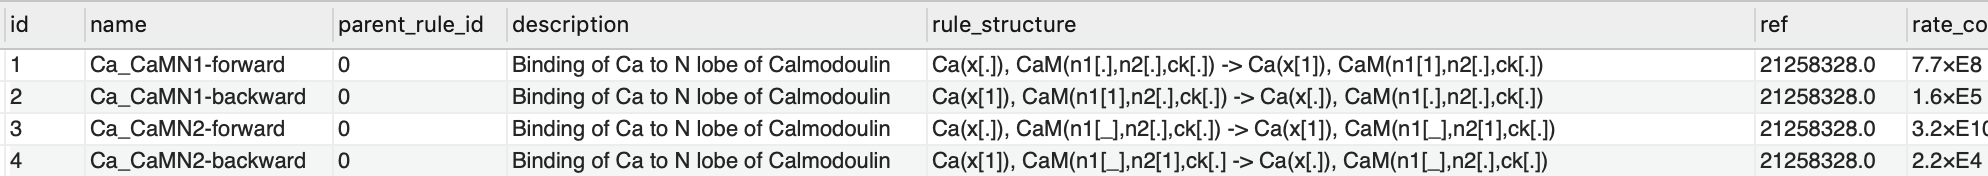
\includegraphics[width=\linewidth,height=14cm,keepaspectratio]{DomainNameOutput1.png}	
		\caption{The retrieved rules from the stored procedure GetRulesFromDomainNamesPair called with the arguments `x' and 'n1'.}
		\label{fig:DomainNameOutput1}		
	\end{figure}

	\item 
\begin{itemize}
	\item 	The stored procedure is called with the domain name arguments `GK,GKBD', using the command, \\
	call GetRulesFromDomainNamesPair(`GK',`GKBD')\\
	from MySQL workbench. 
	\item The expected output is the PPI rules, containing the domain names GK and GKBD within it.
	\item The output obtained from the database contained 9 rows. A snippet of the output is shown below, in figure \ref{fig:DomainNameOutput2}. Each of these PPI rules was verified to contain the domain names GK and GKBD within it.
	\item The stored procedure call was also tested with the arguments swapped (GKBD and GK) and the retrieved rules were verified to be the same.		
\end{itemize}
\begin{figure}[H]
	\centering
	\captionsetup{justification=centering}
	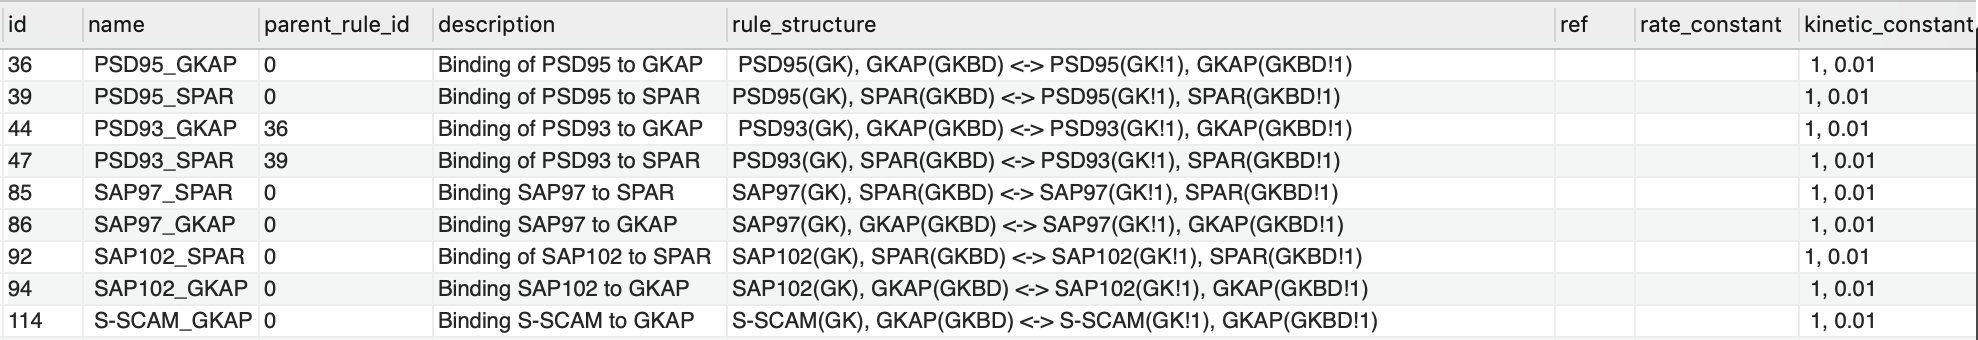
\includegraphics[width=\linewidth,height=14cm,keepaspectratio]{DomainNameOutput2.png}	
	\caption{The retrieved rules from the stored procedure GetRulesFromDomainNamesPair called with the arguments `GK' and 'GKBD'.}
	\label{fig:DomainNameOutput2}		
\end{figure}
\end{enumerate}

\section {Verification of results displayed in UI}
In this section, we proceed to verify the outputs displayed in the UI created using Django and DataTables. To judge the correctness of the results fetched from the database and displayed within the UI, it has to be ensured that the results from the stored procedure are displayed in the UI without any data loss or modifications. This retrieval and display test is performed for obtaining the PPI rules based on both the stored procedures (GetRulesFromAgentName and GetRulesFromDomainNamesPair).

\subsection{Agent Name}
In this test, the stored procedure GetRulesAgentName is called from within the Django app and the output is displayed in the UI. The displayed output in the UI was matched with the output from the stored procedure in MySQL workbench.\\ Two examples of such test cases are as follows:
\begin{enumerate}
	\item The UI is called with the agent name CaM and a snippet of the retrieved rules is shown in figure \ref{fig:CorrectnessAgentName1}. The number of entries retrieved in the UI was 14 and the number of entries retrieved by the stored procedure was also 14. The rules retrieved in the UI were also the same as the ones retrieved by the stored procedure.
	\begin{figure}[H]
		\centering
		\captionsetup{justification=centering}
		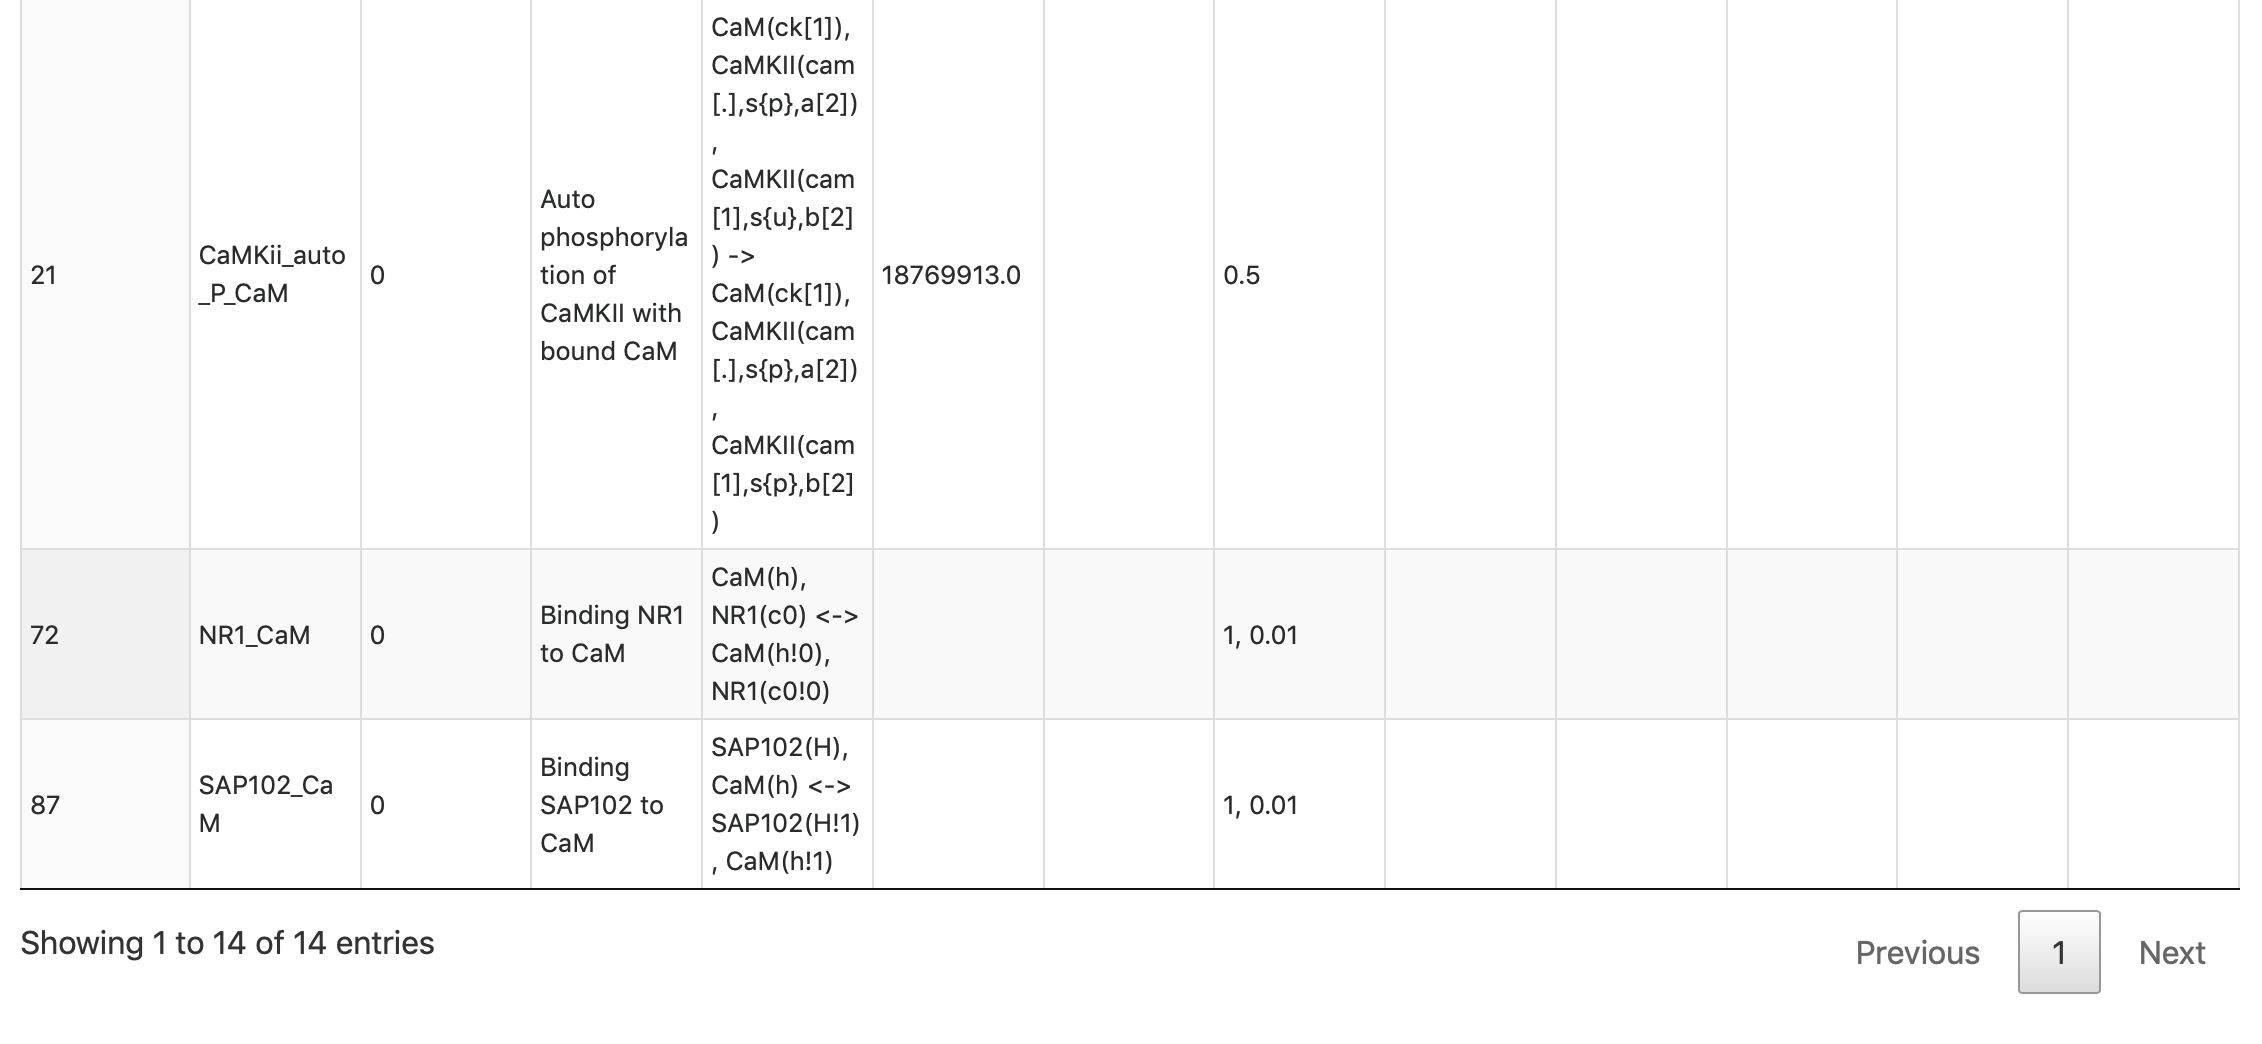
\includegraphics[width=\linewidth,height=14cm,keepaspectratio]{CorrectnessAgentName1.png}	
		\caption{The retrieved rules in the UI obtained by passing the agent name `CaM' as an argument.}
		\label{fig:CorrectnessAgentName1}		
	\end{figure}
	\item The UI is called with the agent name SynGAPa and a snippet of the retrieved rules is shown in figure \ref{fig:CorrectnessAgentName2}. The number of entries retrieved in the UI was 6 and the number of entries retrieved by the stored procedure was also 6. The rules retrieved in the UI were also the same as the ones retrieved by the stored procedure. 
	\begin{figure}[H]
		\centering
		\captionsetup{justification=centering}
		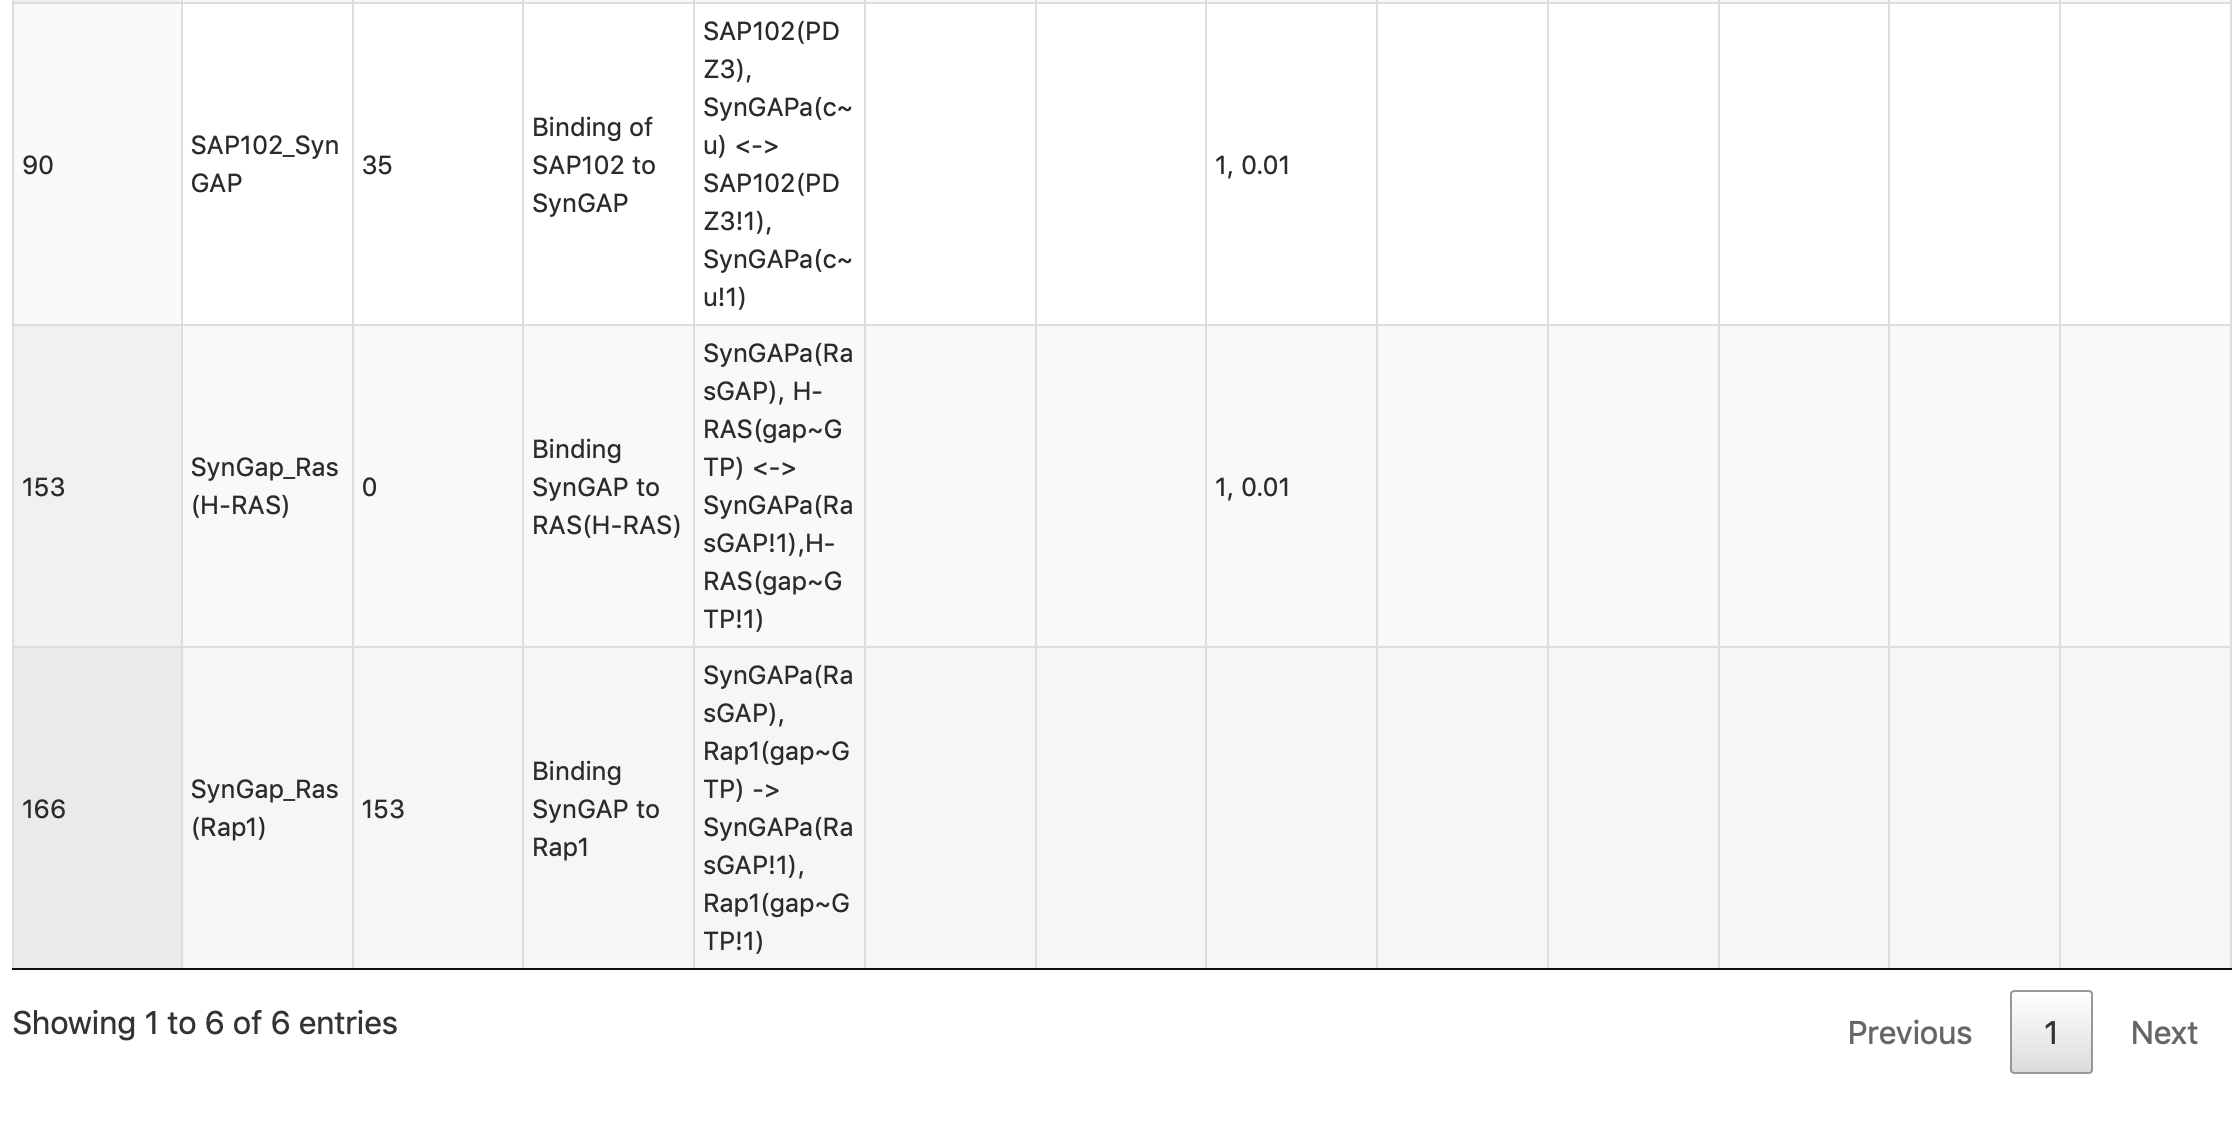
\includegraphics[width=\linewidth,height=6.5cm,keepaspectratio]{CorrectnessAgentName2.png}	
		\caption{The retrieved rules in the UI obtained by passing the agent name `SynGAPa' as an argument.}
		\label{fig:CorrectnessAgentName2}		
	\end{figure}	
\end{enumerate}


\subsection{Domain Names Pair}
In this test, the stored procedure GetRulesFromDomainNamesPair is called from within the Django app and the output is displayed in the UI. The displayed output in the UI was matched with the output from the stored procedure in MySQL workbench. For each of the domain name pair inputs, the entries in text boxes of the web form were interchanged the and results were verified to be the same.\\ Two examples of such test cases are as follows:

\begin{enumerate}
	\item The UI is called with the domain names x,n1 and a snippet of the retrieved rules is shown in figure \ref{fig:CorrectnessDomainName1}. The number of entries retrieved in the UI was 4 and the number of entries retrieved by the stored procedure was also 4. 
	The rules retrieved in the UI were also the same as the ones retrieved by the stored procedure. 
	\begin{figure}[H]
		\centering
		\captionsetup{justification=centering}
		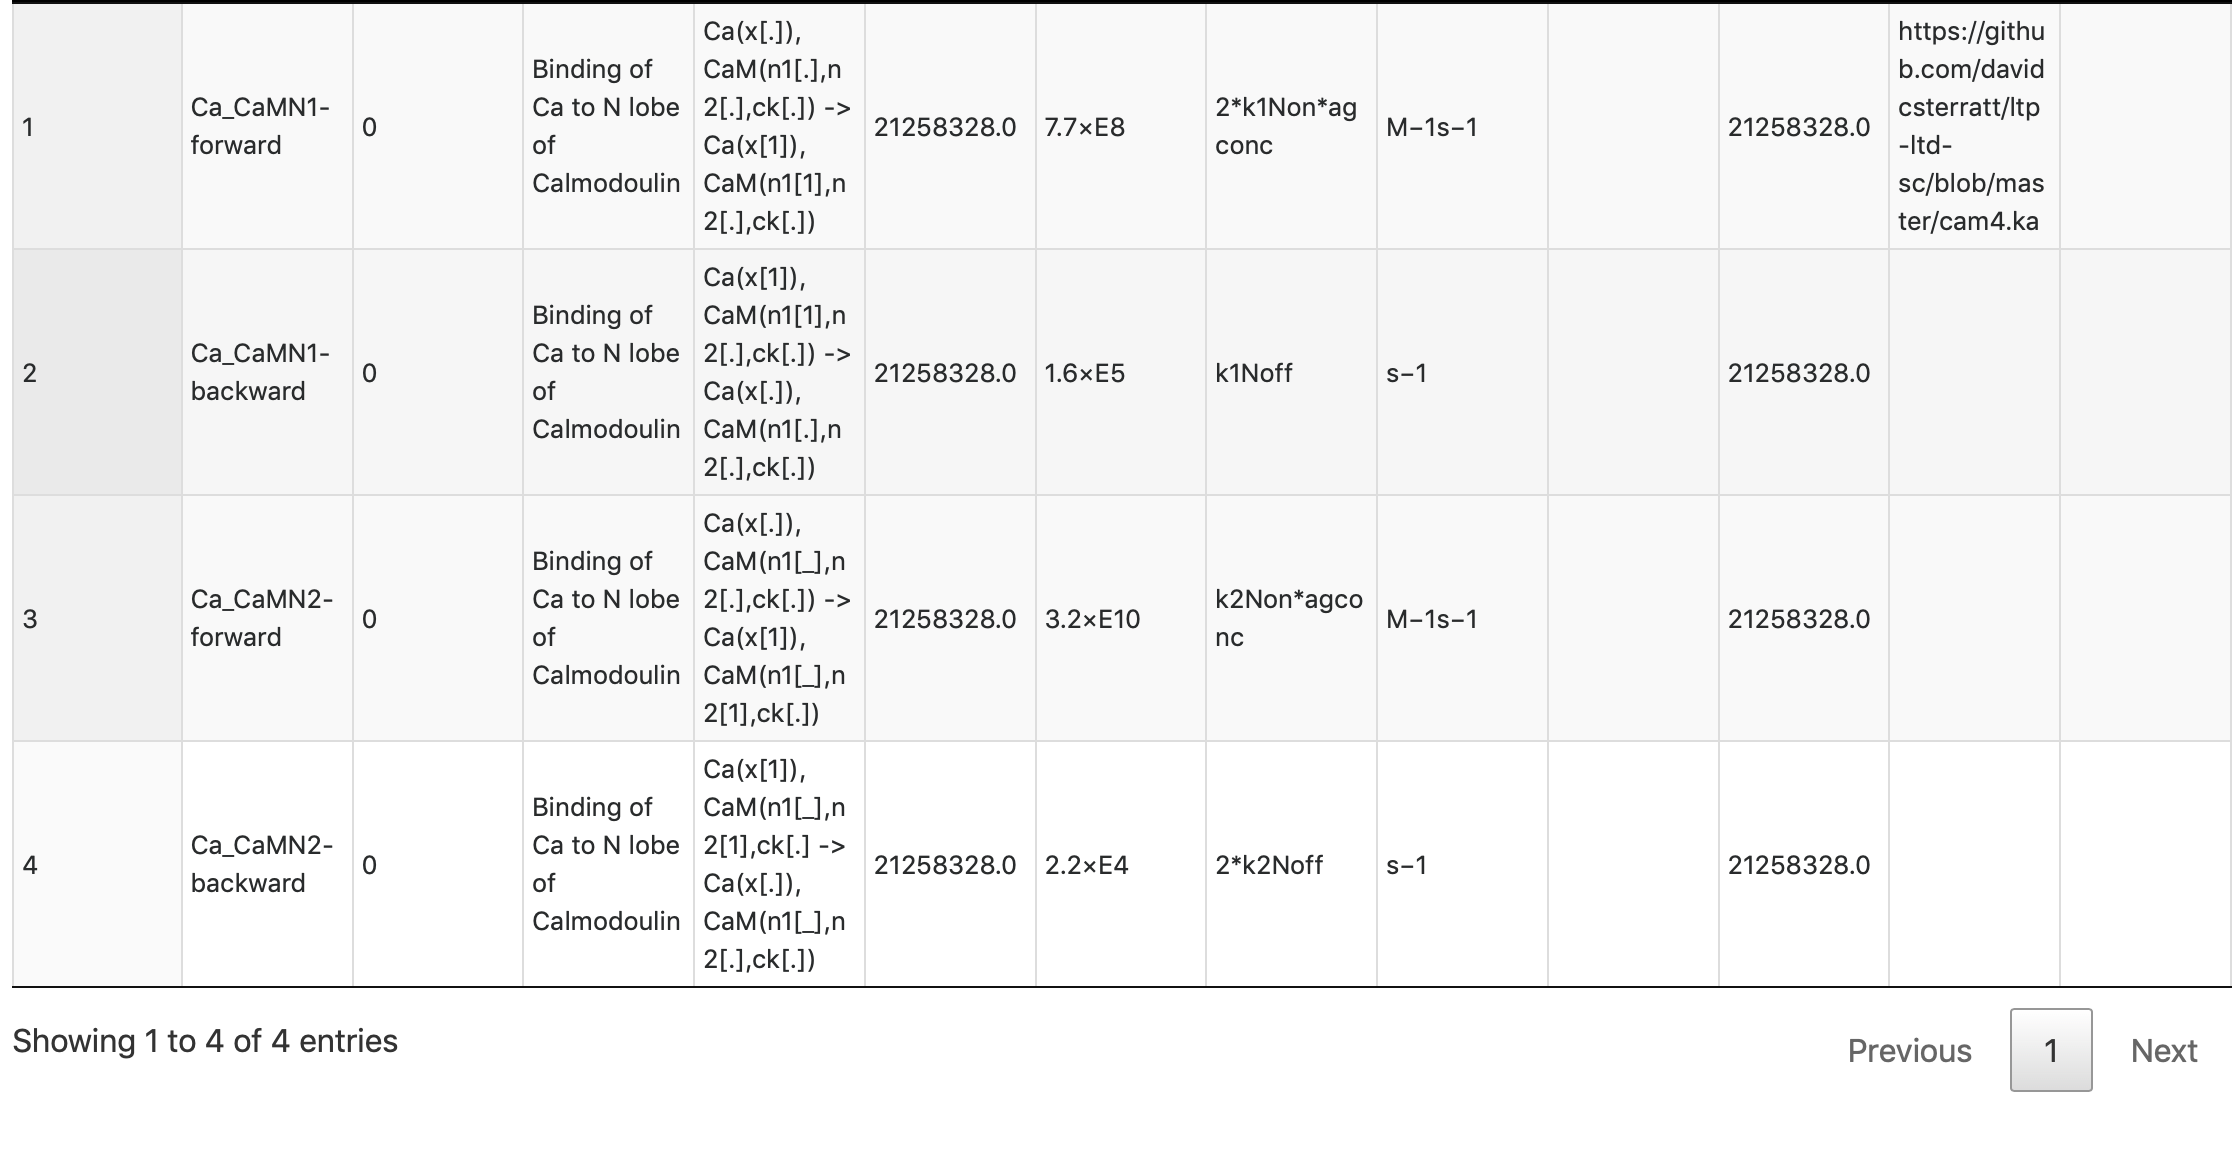
\includegraphics[width=\linewidth,height=14cm,keepaspectratio]{CorrectnessDomainName1.png}	
		\caption{The retrieved rules in the UI obtained by passing the domain names `x' and `n1' as arguments.}
		\label{fig:CorrectnessDomainName1}		
	\end{figure}
	\item The UI is called with the domain names GK,GKBD and a snippet of the retrieved rules is shown in figure \ref{fig:CorrectnessDomainName2}. The number of entries retrieved in the UI was 9 and the number of entries retrieved by the stored procedure was also 9. The rules retrieved in the UI were also the same as the ones retrieved by the stored procedure. 
	\begin{figure}[H]
		\centering
		\captionsetup{justification=centering}
		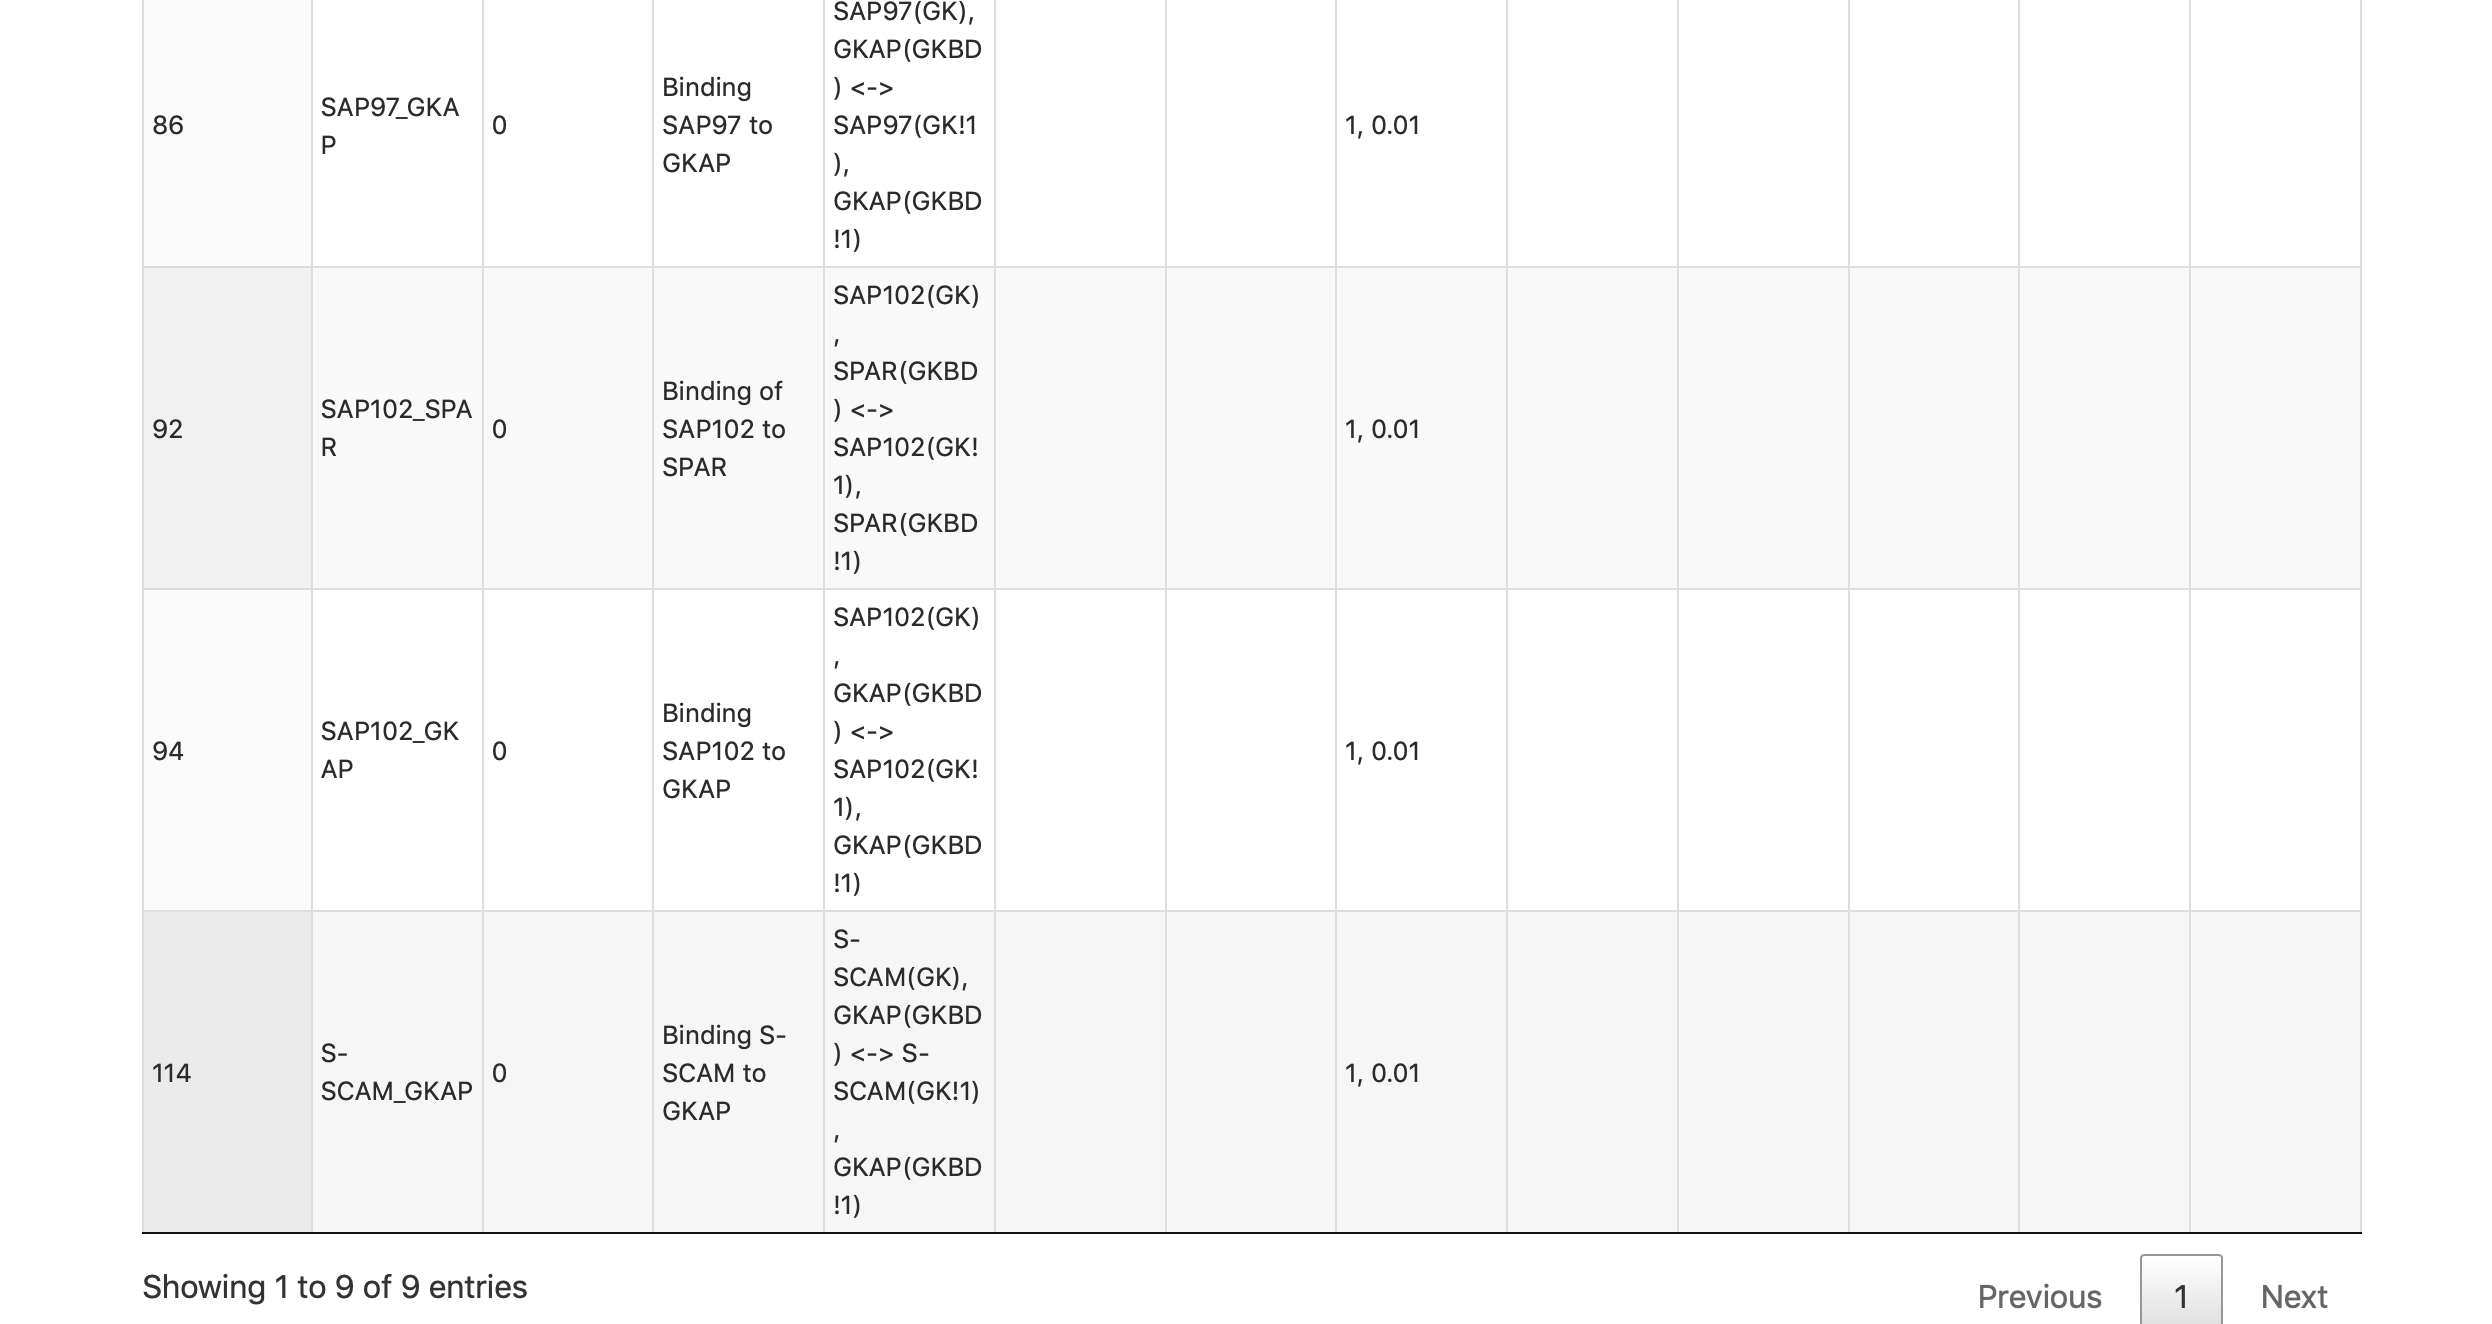
\includegraphics[width=\linewidth,height=6.5cm,keepaspectratio]{CorrectnessDomainName2.png}	
		\caption{The retrieved rules in the UI obtained by passing the domain names `GK' and `GKBD' as arguments.}
		\label{fig:CorrectnessDomainName2}		
	\end{figure}	
\end{enumerate}

\section{KaSim output example}
The Kappa rules may be fed to a Kappa simulator to generate a visualization of the protein interaction rules. For a demonstration, this section presents an example of feeding the Kappa rules to KaSim, the web simulator \cite{KaSimBrowser}. The rules fed to the simulator are depicted in the left-hand side and the output obtained is on the right-hand side of figure \ref{fig:kappaOutput}. 
	\begin{figure}[H]
	\centering
	\captionsetup{justification=centering}
	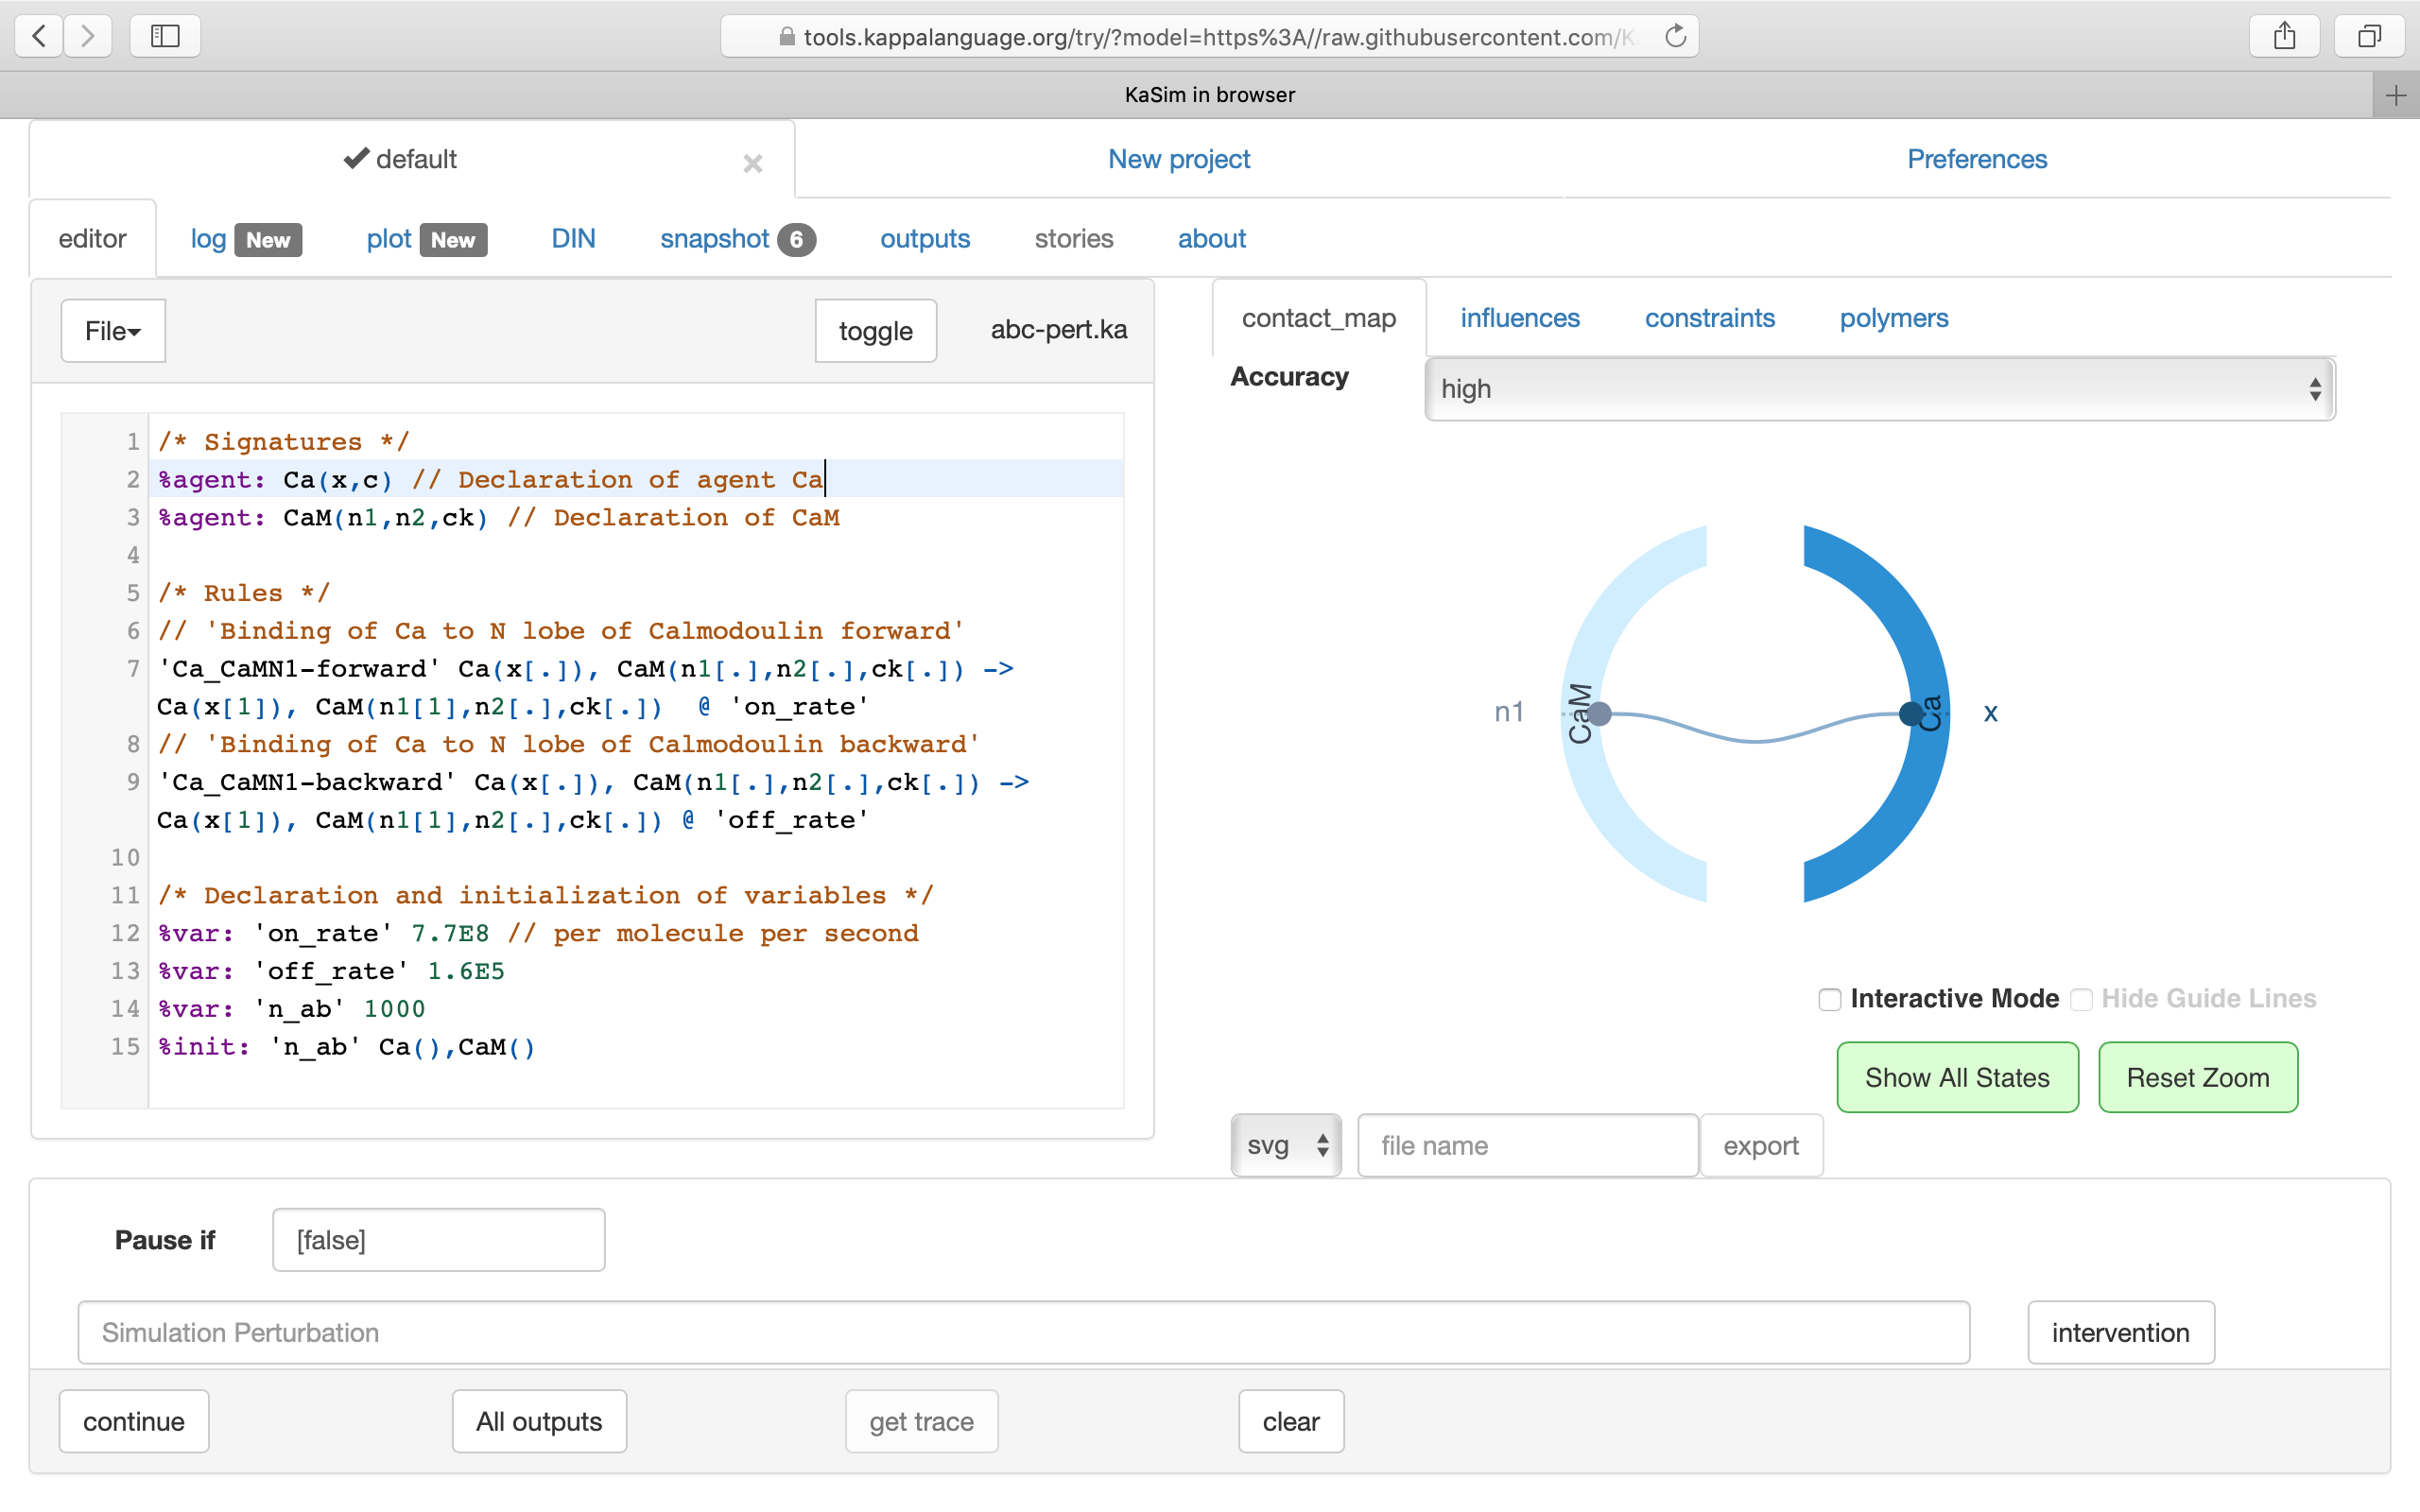
\includegraphics[width=\linewidth,height=8.5cm,keepaspectratio]{KasimOutput}	
	\caption{An example of PPI rules visualization by KaSim \cite{KaSimBrowser}}
	\label{fig:kappaOutput}		
\end{figure}	

\chapter{Conclusion and Future Work}
This chapter summarizes the aims and objectives achieved through this project. It also lays down certain suggestions for future work in this field.

\section{Conclusion}
The purpose of this project was to create a central repository for protein-protein interaction rules, stored in the rule-based (Kappa) format. These rules were collected by researchers from previous research and provided as raw data, to be processed and saved to the database. The database was built as per requirements discussed with the project supervisor and tested to ensure correctness. 

This project achieves the aforementioned purpose by the successful creation of the centralized database for storing the protein-protein interaction rules. The design of the database is such that, it is flexible to accommodate future changes and additions of PPI rules. Rule additions can be made to the database as per steps laid out in Section 3.2.

The stored procedures created within the database, as part of this project, help in extracting the PPI rules based on either agent name or a pair of domain names. The stored procedures are helpful as they provide ready access to a set of SQL queries that enable filtering of the PPI rules. 

On discussions with the project supervisor and keeping in mind the future direction of the project, it was decided to create a web application with a user interface (UI) to access the PPI rules. Although the creation of the web application and UI were not part of the original project proposal, it was decided to extend the work to improve accessibility and accommodate the future direction of the project. Hence, the original proposal was further extended significantly.

In the web interface, the PPI rules are obtained based on agent name or domain names pair, by making calls to the stored procedure routines within the database. The web application and user interface, allow users to access the PPI rules in a user-friendly format. The UI options in the user interface allow users to preserve the results displayed in the tables, onto their local system. This can be achieved as the results displayed in the UI can be exported to different file formats like CSV and Excel.  
\section{Future Work}
A possible area of future extension to the database may be, to include a rule class for the rules stored in the PPI database. This class would help emphasize the priority of a protein-protein interaction rule. A higher priority rule would be the one having greater certainty and more information.

Another area of development could be to create and include more stored procedures in the database. These stored procedures could help in further filtering the PPI rules. For example, the existing stored procedure for extracting PPI rules based on domain name pairs could be extended to include an open and closed universe. In an open universe, the protein interaction rules could contain the pair of domain names besides containing other domain names. However, in a closed universe, the protein interaction rules retrieved by the stored procedure would only contain those two domains. Depending upon the project requirement, this can be created by either including a universe indicator in the existing stored procedure or creating separate stored procedures, one for each universe.

Also in the area of scripting, scripts can be written to process the rules obtained from the UI in the form of Excel or CSV files. The processing can be such that it renders the rules ready for being fed to the simulator for visualization of the protein interactions.


%\section{Final Reminder}

%The body of your dissertation, before the references and any appendices,
%\emph{must} finish by page~40. The introduction, after preliminary material,
%should have started on page~1.

%You may not change the dissertation format (e.g., reduce the font
%size, change the margins, or reduce the line spacing from the default
%1.5 spacing). Over length or incorrectly-formatted dissertations will
%not be accepted and you would have to modify your dissertation and
%resubmit.  You cannot assume we will check your submission before the
%final deadline and if it requires resubmission after the deadline to
%conform to the page and style requirements you will be subject to the
%usual late penalties based on your final submission time.


\bibliographystyle{plain}
\bibliography{mybibfile}

%% You can include appendices like this:
 \appendix
% 
\chapter{Software Version}
% 
This section includes software versions that were used to create and deploy the application onto a local machine. While deploying to a database/web server it may be helpful to have these details.
 \section{Operating System}
 macOS Mojave Version 10.14.2\\
 Obtained by checking details of the Operating System.
 \section{MySQL Version/ Client Version}
 MySQL version: 8.0.16\\
 MySQLWorkbench version (8.0): Version 8.0.16 build 14498383 CE(64 bits) Community\\
 Both of these details are obtained from within MySQLWorkbench.
 \section{Python Version}
 Python 3.7.0\\
 Obtained by the command: python --version
 \section{MySQL Connector Version in Python scripts}
 8.0.16\\
 This is obtained as a property of the mysql.connector module.
 To check the version:
 Create a python script with the following details:\\
 import mysql.connector\\
 print(mysql.connector.\_\_version\_\_)\\
 \section{Django Version}
 2.2.3\\
 To check the django version navigate to the project folder and use the manage script.\\
  Obtained by the command: python manage.py version
 \section{Data Tables Version}
 1.10
 
\end{document}
